\chapter{The models and results \label{chapter:models}} 

\section{Introduction}

\subsection{Organisation of the chapter}

This chapter presents results from the model framework. It does this in five sections with the following aims:

\begin{itemize}
	\item Test that the main economic components of the model function correctly, first without any spatial element, and then with space costs included
	\item Test the difference between using a `greedy' vs 'constrained' utility approach.
	\item Test how Actors react to changes in both spatial and non-spatial variables, given different model setups.
	\item Investigate the issue of connecting economic components, moving towards a `general' model
	\item Test outcomes for a model connecting production to welfare.
\end{itemize}

\subsection{Presentation of results \label{sec:resultspres}}

Results are presented in three ways:

\begin{itemize}
	\item Model run results:
\begin{itemize}
	\item $(1)$ Visualisation of model run
	\item	$(2)$ Chosen data output from model run
\end{itemize}
	\item $(3)$ Analytic results
\end{itemize}

The detail of visualisations vary, so it is best to leave a full description of them for the sections in which they are used: details will be given in the figure captions. These aim to give an initial intuitive sense of what the model is showing, before going on to present the relevant data output. The visualisation can be as good a data summary as graphed data output, since it can be easier to see what is fundamentally happening through these than in the data, in much the same way that any map can enable a good overview.

A more mathematical analysis is used in two types of situation. Firstly, many of the basic dynamics of the model are best communicated using an analytic approach. Secondly, when the model framework produces results that require further explanation. When the agent model outputs a particular outcome, is it due to Actors acting rationally? If so, what factors are at work? The framework proposes these questions, but a full answer may require an analytic comparison. Where results of such an comparison are informative, they have been  included in this chapter. As discussed in the conclusion, this is a happy synergy: the  agent model helping to highlight possible lines of inquiry, and an analytic approach  shedding further light on the issues.

It will be made clear in the text where a model output or analytic approach is being discussed.

\section{Testing utility functions \label{sec:testingutils}}

%%%%%%%%%%%%%%%%%%%%%%%%%%%%%%%
% Scenario table
%%%%%%%%%%%%%%%%%%%%%%%%%%%%%%%
\renewcommand{\arraystretch}{1.2}
\begin{table}[!hbt]
\begin{center}

%\begin{tabular*}{0.8\textwidth}{|l|l|}
\begin{tabular}{|l|l|}
\hline 
\textbf{Component} & \textbf{Description}\\
\hline
Run type & Single runs, arbitrary number of days\\
\hline
Actor type & Single Person, small number of Firms\\
\hline
Actor action & Firms: static sources of goods \\
& People: spend set wage only\\
\hline
Space-type & None: space excluded \\
\hline
Parameters & Fixed: wage, price of good\\
\hline
Utility form & See sections\\
\hline
Production form & None: demand always met\\
\hline

\end{tabular}

\caption{Model components for `Testing utility functions' \label{tab:utiltests}}
\end{center}
\end{table}

This section demonstrates that the model framework successfully replicates the basic micro-economic ideas outlined in chapter \ref{chapter:location}. This is done by initially excluding any spatial elements to keep a clear focus on the central economic functions themselves.
\subsection{CES function}

The discrete-good \gls{ces} function \eqref{eq:-6} is most commonly used in the models that follow. Section \ref{sec:cesspace} explores the interaction of the \gls{ces} function with space; the function's basic output is tested here. 

The following uses a model run test (see figure \ref{fig:CEStestResults}) that removes all spatial costs and normalises wage to 1 and all good costs also to 1. A single Person then optimises: what optimal mix of goods can they buy? Firstly, this is done for $0<\rho<1$, in a situation with two goods. (Recall that as $\rho \rightarrow 1$, goods become substitutes and \gls{lov} drops.) Two views of that data are given, since for $\rho<0.2$, utility becomes very large. Secondly, $\rho$ is held at $0.75$ and the number of goods (in the model, the number of supplying Firms) is changed, up to a thousand. While the budget constraint does stop utility from growing exponentially with varieties, it does not level off. If a Person were able to split their own time into infinite slices and produce them all in their own backyard, they could increase their utility infinitely. 

\begin{figure}[h!]
\centering
\subfloat[2 goods, $\rho$ changed]{\label{fig:ces12}\includegraphics[width=0.4\textwidth]{ChapterModels/Figures/CES2firm_rhochange1}}
\hspace{0.1}  
\subfloat[2 goods, $\rho$ changed, from $\rho=0.2$]{\label{fig:ces13}\includegraphics[width=0.4\textwidth]{ChapterModels/Figures/CES2firm_rhochange2}}
\hspace{0.1}  
\subfloat[$\rho=0.75$, good number changed]{\label{fig:ces11}\includegraphics[width=0.4\columnwidth]{ChapterModels/Figures/CES_rho075_firmchange}}%
\caption{Testing CES function works correctly. \ref{fig:ces12} and \ref{fig:ces13} look at the same data: two goods, changing $\rho$. \ref{fig:ces11} keeps $\rho$ fixed at 0.75 and changes the good number. \label{fig:CEStestResults}}%
\end{figure}


\subsection{Cobb Douglas}
%Just occurs to me: these are really tests for the greedy al. Not a surprise that the constrained should work, is it? Or is it? Who knows?

Actors with a Cobb Douglas utility function \eqref{eq:-3} want to buy a mix of two goods $F$ and $M$, where $p_F$ and $p_M$ are the price of $F$ and $M$ respectively. The constrained optima \eqref{eq:optCDF} and \eqref{eq:optCDM} were described in section \ref{sec:constrained}.  repeated here:

\begin{equation}
F=\frac{\delta Y}{p_F}\label{eq:optCDF}
\end{equation}
 
\begin{equation}
M=\frac{(1-\delta) Y}{p_M}\label{eq:optCDM}
\end{equation}

The Cobb Douglas share parameter $\delta$ exactly describes the income for each sector producing $F$ and $M$. Price-setting does not affect the income of the seller at all: each always gets exactly a $\delta$ share. In the \gls{coremodel}, this feature of the Cobb Douglas is useful, since it rules out any elasticity between the two sectors of manufacturing and food, keeping the analysis much simpler. 

The fact that the share parameter $\delta$ dictates each sector's income can be seen analytically from \eqref{eq:optCDF} and \eqref{eq:optCDM}: the price of each is internal to its own optimum and does not appear in the other. Therefore, changing the price of one \emph{cannot} affect demand for the other. Each sector is independently unit elastic: if the price is dropped, demand will rise - but such that the total revenue remains the same.

%Not always true, depends on rev. Oh - just thought, that's a useful test for DMR. If no cross-elasticity, can isolate, see if DMR improves.
Putting this into an agent context, however, if Firms are being asked to take price decisions, they will find they have no effect, removing their ability to make optimising decisions. This can have a spatial consequence. In a situation where only two firms exist and space costs are internal to them, each producing one of $F$ and $M$, they can gain nothing by changing their location: their income will stay precisely the same. Any reduction in space costs will lower costs, which will lower prices, but this will be exactly balanced by raised demand.

\begin{figure}[h!]
\centering
\subfloat[2 Firms randomise prices]{\label{fig:CDrand1}\includegraphics[width=0.4\textwidth]{ChapterModels/Figures/CD_random1}}
\hspace{0.1}  
\subfloat[Income change for 2 Firms: none]{\label{fig:CDrand2}\includegraphics[width=0.4\textwidth]{ChapterModels/Figures/CD_random2}}
\caption{2 Firms facing Cobb-Douglas demand randomise prices (\ref{fig:CDrand1}): no effect on either of their revenue (\ref{fig:CDrand2}). \label{fig:CD_2firm_randomPricing}}%
\end{figure}

Figure \ref{fig:CD_2firm_randomPricing} shows data from an agent model run where two firms set random prices for $F$ and $M$. It can be seen that both firm's income levels stay the same regardless of price. Price elasticity of demand, then, is unit elastic: any change in price is matched by a change in demand that keeps revenue levels static. This is as should be expected from Cobb Douglas utility. 

\begin{figure}[h!]
\centering
\subfloat[Optimal demand for goods 1, 2]{\label{fig:CDfix1}\includegraphics[width=0.4\textwidth]{ChapterModels/Figures/CD_opt1}}
\hspace{0.1}  
\subfloat[Price change of Firm 2]{\label{fig:CDfix2}\includegraphics[width=0.4\textwidth]{ChapterModels/Figures/CD_good2cost}}
\caption{Two Firms selling goods 1 and 2: Firm 1's price fixed, 2 attempting to optimise price. Actors with Cobb Douglas utility: changing price of one has no effect on demand for the other \label{fig:CD_1fixed}}%
\end{figure}

Figure \ref{fig:CD_1fixed} makes the same point in a different way: it shows the outcome when one firm's prices are fixed while the other attempts to find a revenue-maximising price. As mentioned above, this fails because they can affect no change on their revenue in this situation. For the fixed-price firm, actors consume a constant amount - and that is not altered by changes in the price of the other good. This shows that actors' demand for each is independent of the other. 

Note that, in situations where delivery costs `melt away' or total model revenue has any other leak-points, the above would not hold: Firms could, for instance, improve their revenue by increasing proximity to their market, if expenditure on delivery costs went elsewhere.

An interesting point arises from implementing the Cobb Douglas in agent form. Imagine a situation where only the agent-based approach to testing the utility function existed. Eventually, the independence of the two sectors in the Cobb Douglas would become apparent. But how would one be able to `explain' it? It is hard to imagine any answer that would not eventually reduce to the analytic result from the Lagrangian optimisation. Equations \eqref{eq:optCDF} and \eqref{eq:optCDM} appear to be the best possible explanations for what happens - a solution that the murkier agent approach would perhaps have made considerably more difficult to discern. Conversely, it is clear that Cobb Douglas utility \emph{imposes} this strict unit elasticity on sectors. As with the \gls{coremodel} this may be desirable, but it underscores the interdependence between Firms and People discussed in section \ref{sec:decstruct}. This is not necessarily an argument against \gls{abm}, since - as the rest of the chapter discusses - the flexibility of the method has other advantages. But it does highlight that, for many problems, neither method has a unique claim to explanatory power.

%What else to say about the Cobb Douglas? Come back and stick in an example of externalities for space costs, problems for 'general' analysis.
\subsection{Engel Function \label{sec:engeltest}}

The Engel function breaks with the previous two utility functions: changes in costs \emph{do} affect actors' choices, and the level for each consumed good. Use of the constrained optima for the Engel function has a problem, however: it can produce negative values. This is clear enough from the constrained equation for $M$, \eqref{eq:EngelpriceoptM}:

\begin{equation}
M=\frac{Y(1-\delta)}{p_{M}}-\delta\gamma
\end{equation}
 
Let the wage $Y = 1$, the share parameter $\delta = 0.5$ and the price of $M$, $p_{M}=1$: it then just becomes $M = 0.5 - 0.5\gamma$. So, for $gamma > 1$, demand for $M$ is below zero. Subfigure \ref{fig:engelTest1} shows the result from letting a model agent use the constrained function: not only does negative demand result, it means demand for the necessity good is incorrect.

\begin{figure}[h!]
\centering
\subfloat[]{\label{fig:engelTest1}\includegraphics[height=40mm]{ChapterModels/Figures/EngelWithoutCorrection}}%
\hspace{0.2}  
\subfloat[]{\label{fig:engelTest2}\includegraphics[height=40mm]{ChapterModels/Figures/EngelWithCorrection}}%
\caption{Constrained Engel function, with and without correction for negative consumption value. Demand for necessity (nec), luxury (lux) and utility (av utility) on y axis, wage on x axis. \label{fig:engelCorrection}}%
\end{figure}

The simple solution is just to test for when the constrained approach finds $M<0$. All that needs to happen under those circumstances is the following:

\begin{itemize}
	\item Find what was spent on $M$ - just $M \cdot P_m$. This will be a negative amount
	\item Reassign the spend to $F$. Because it is negative, demand for $F$ will be less.
	\item Set $M$ to zero.
\end{itemize}

The model-run result is sub-figure \ref{fig:engelTest2}, which produces economically sensible demand for both goods: below the point where $M$ would become negative, the spend is redirected to $F$.

In contrast, if the goods go through the Engel function via the greedy algorithm, it cannot find itself in the same negative demand situation: by design, it works with the available amount of goods. This means, as shown in figure \ref{fig:engeltest_income1to2}, that below the point where demand for the luxury good begins, necessity demand acts sensibly. Note, however, that it does not perfectly match the analytic result: the greedy utility has a certain amount of noise (see below in section \ref{sec:greedyvsconstrained} for related tests). One result of this is that where usually no demand for the luxury good should be present, there is a slight amount. (The noise level here is quite high for illustration: greedy algorithm iteration number is low.)

\begin{figure}[h!]
\centering
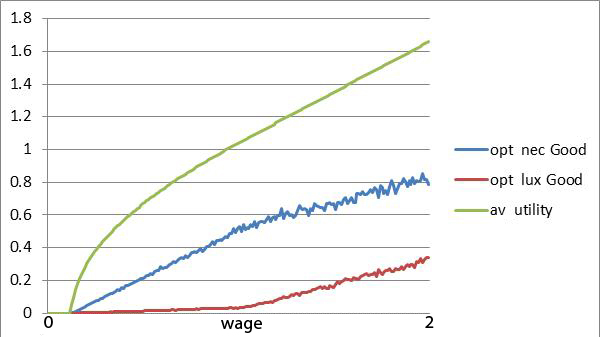
\includegraphics[width=0.4\columnwidth]{ChapterFramework/figures/engeltest_income1to2copycopy}%
\caption{Testing the Engel utility function: $\gamma = 1$, wage level changed from 0 to 2. Graph shows optimal amount of necessity and luxury good plus utility on the y axis, and wage on the x axis. \label{fig:engeltest_income1to2}}%
\end{figure}

In both constrained and greedy optimisations, then, Actors can replicate the most important feature of the Engel function: when incomes are low (below the level set by $\gamma$, given unit prices), they demand only the necessity good (plus some small extra amounts of luxury good resulting from small random fluctuations in the case of the greedy optimisation routine). The constrained optimisation can achieve the same thing with much less noise, but requires a correction in the algorithm to `reallocate' any negative spend.

The next section looks in more depth at the different between the constrained and greedy algorithm approach to utility.

\section{Greedy versus constrained utility \label{sec:greedyvsconstrained}}

Chapter \ref{chapter:ABM} argued that utility is a useful concept for describing how people react to cost changes. In the model framework, two different approaches are tested for modelling People's utility: a `greedy' algorithm (see section \ref{sec:optimisingbundles}) and a more economically traditional constrained utility function, of the type outlined in section \ref{sec:constrained}.

What might be the problem in using constrained utility in an agent model? Section \ref{sec:rationality} pointed out that constrained utility is, as Leijonhufvud noted, ``a statement about actual performance, not just motivation''. The constrained function takes in a budget amount and goods prices and outputs an amount of demanded good. But what if the demanded good is not available? An `objective function' of this sort appears unable to deal with this situation. Consider the equation \eqref{eq:CESconstrained}, the constrained optima for an $n$-good \gls{ces} function described in section \ref{sec:constrained}. For a Person with a bundle of detected goods, the optimal amount for each good $c_j$ is given by:

\begin{equation}
c_j = \frac{p_j^\frac{1}{\rho-1}Y}{\sum_{i=1}^{n}p_i^\frac{\rho}{\rho-1}} \label{eq:CESconstrained2}
\end{equation}

 - where $p_j$ is the price of good $c_j$, $Y$ is the budget, and the denominator sums the price of each good raised to $\rho/\rho-1$. What happens in a situation where, for example, $c_1 = 1$ but only $0.5$ is available? There is then a different problem to solve: what is the optimal amount for the other goods, given that we know the available stock of  $c_1 = 0.5$. The constrained optima from equation \eqref{eq:CESconstrained} provides only demand as an output. There is no way to include a set demand amount for one or any of the goods; the function is simply not set up that way, and cannot be due to its roots in constrained optimisation. Neither is it quite as easy as removing $c_1$ from the list and recalculating, since demand for each affects all the others.

On the surface, the greedy algorithm approach appears a more plausible approach to utility: People weigh up a given mix of goods, and compare until they find what makes them `happiest' (that is, what gives them the highest utility). They do not have a superhuman constrained function informing them of their optimal demand. If any good is not available in the quantities they want, budget slices can be reassigned to the pot for the next iteration. In practice, however, this literal approach to stock consumption is complex to implement - not from the demand side, but because Firms then need to find some way to produce the \emph{correct} amount of stock given demand signals.

Fowler's approach is to make a tactical modelling choice that avoids the need to consider rationing of limited goods: ``workers select their optimal bundle of goods without reference to the actual supply of the good'' (\citealt{fowler_finding_2011} p.10). Thus, they still have an `objective' demand level. He notes a key informational advantage: this sends ``clear signals to firms about the actual level of demand for their goods at the current price'' (ibid.) As he says, it also avoids having to work out any explicit rationing strategy if several actors are competing for limited goods. 

While this is an effective simplification, it may be problematic depending on what the goal is. For instance, what exactly does it mean for Firms to receive demand signals for goods that People could not actually acquire? This is saying, `I wanted more than was available', and so in theory a Firm can use that information to inform their production decisions. This is a feasible approach if stock is theorised in a particular way; section \ref{sec:prodtowelfare} presents a model that does this.

On a more mundane level, however, it is useful to compare the greedy algorithm to its constrained counterpart, to show that the two produce almost identical results. They are only different to the extent that the greedy algorithm cannot avoid a certain quantity of noise; section \ref{sec:engeltest} discussed how noise can affect utility outcome. Noise in utility is also put to good use in the model presented in section \ref{sec:firmsLoV} to examine how it impacts on Firms' ability to make appropriate decisions. The next section looks at the two approaches to utility maximisation in more detail.

%Section \ref{sec:optimisingbundles} explained that People assemble a set number of `Bundles' of goods, and work out the utility for each. They then select the highest utility bundle. 
 %I think. Better work out if that works. 
%There is, however, the problem of `objective demand' in a world that may not have the stock to meet it. One way to address this is to allow a Person to work with the stock that \emph{is} available. This can be done using the `greedy algorithm' approach...

\subsection{Comparing the two}

How do the two approaches compare when stock levels are not an issue? In model runs, they produce almost identical results. Figure \ref{fig:GreedyVsConstrained} shows both the constrained and greedy algorithms optimising two and eight goods as delivery costs are increased. Sub-figure \ref{fig:gnc5} compares the difference in utility levels: the greedy algorithm does not quite match the accuracy of the constrained, but gets very close.
%The more important difference between them is computational: the greedy algorithm is much more computationally expensive. 

The exact level of difference between the constrained optima and the greedy algorithm depends on the number of iterations the latter is given to ratchet towards utility-improving budget slices. Figure \ref{fig:GreedyItes} shows what difference the iteration number makes for two scenarios. Both show aggregate statistics for a thousand optimisations at each iteration-number point, up to 2000. Again, it is a \gls{ces} function at $\rho=0.5$, all good costs are even and the budget is one. This means the `correct' optima for a single good is known. For the first example (\ref{fig:gi1} and \ref{fig:gi2}) optimising two goods, that is 0.5 for each, and as expected the constrained method finds this. Very low iteration numbers do not, on average, manage to get very close to this optimum, but by the time 1000 iterations are used, it is missing the perfect optima only minimally. Sub-figure \ref{fig:gi2}, however, shows that further improvements - though tiny, note the y-axis values - do continue to be made for iteration increases up to 2000 (in this example). There is always a little noise left in comparison to the constrained method.

The last sub-figure (\ref{fig:gi3}) shows the same outcome if eight goods are used - again showing results for one of those goods, whose analytic optima is 0.125. It is a quirk of the method that a higher number of goods can be optimised more quickly. The basis for this is an effect from good number: budget slices are all individually smaller: there is simply less scope for large variation due to the randomisation method used.

\begin{figure}[h!]
  \centering
  \subfloat[]  {\label{fig:gnc1}\includegraphics[width=0.4\textwidth]{ChapterModels/Figures/avUtilityConstrainedcopy}}
  \hspace{0.1}    
  \subfloat[]  {\label{fig:gnc2}\includegraphics[width=0.4\textwidth]{ChapterModels/Figures/avUtilityGreedycopy}}
  \hspace{0.1}    
  \subfloat[]  {\label{fig:gnc3}\includegraphics[width=0.4\textwidth]{ChapterModels/Figures/allUtilityConstrainedcopy}}
  \hspace{0.1}    
  \subfloat[]  {\label{fig:gnc4}\includegraphics[width=0.4\textwidth]{ChapterModels/Figures/allUtilityGreedycopy}}
  \hspace{0.1}    
  \subfloat[Difference between greedy (G) and constrained (C)]  {\label{fig:gnc5}\includegraphics[width=0.4\textwidth]{ChapterModels/Figures/diffAvUtilGnCcopy}}
  %\hspace{0.1}    
  \caption{Comparing greedy and constrained utility algorithms, fixed People, fixed Firms supplying goods at random distances at give a spread of values. Space costs on all goods increased from left to right. \label{fig:GreedyVsConstrained}}
\end{figure}

\begin{figure}[h!]
  \centering
  \subfloat[1 of 2 goods, zero to 2000 iterations]  {\label{fig:gi1}\includegraphics[width=0.4\textwidth]{ChapterModels/Figures/greedyites1}}
  \hspace{0.1}    
  \subfloat[1 of 2 goods from 1100 iterations]  {\label{fig:gi2}\includegraphics[width=0.4\textwidth]{ChapterModels/Figures/greedyites2}}
  \hspace{0.1}    
  \subfloat[1 of 8 goods, zero to 2000 iterations]  {\label{fig:gi3}\includegraphics[width=0.4\textwidth]{ChapterModels/Figures/greedyites3}}
  \caption{Greedy algorithm optimising 2 goods (\ref{fig:gi1} and \ref{fig:gi2}) and 8 goods (\ref{fig:gi3}). Optimum for one good is shown. 1000 optimisations for each iteration point, mean and one standard deviation.  \label{fig:GreedyItes}}
\end{figure}

The difference between the greedy and constrained algorithm is a useful way for thinking about the issue of realism and descriptive mapping in model structures, and the use of analytic optimisation more generally. Chapter \ref{chapter:ABM} discussed the centrality of equilibrium to neoclassical economic analysis, and the criticisms of agent modellers. Equilibrium skips to the end-point of a process: what about the process itself? 

Compare the underlying method of constrained versus greedy approaches to utility. Section \ref{sec:constrained} explained that the process of acquiring the constrained utility equations is to put them through a Lagrangian optimisation, where an algebraic budget is used to constrain the raw utility function. This effectively ditches the original utility and budget functions and replaces them with a third set of equations able to give optimal good quantities from an actual budget value and a set of good prices. In the model framework, as section \ref{sec:optimisingbundles} explained, those constrained equations work well since individual Good costs and People's budgets can be passed in, and optimal quantities of good returned. 

Once those values are found, however, the Person's utility level is still unknown. In terms of realism, this is a somewhat `spooky' outcome: the Person has their optimal quantities but does not know how happy it makes them. To get that information out of the model, the optimal good quantities must be fed \emph{back through} the original utility function. Causally, that makes no sense: a Person uses some function to find the good quantities they want, and then works out precisely how well off it makes them \emph{after} they have identified their optimal bundle.

In contrast, the greedy algorithm seems more `plausible', and certainly coheres more to the real-world process of decision-making. People must `hold up' bundles of goods and test the utility of each. Yet the greedy and constrained approach are clearly producing the same result, both succeeding at homing in on the point where the function can no longer change. However, the analytic constrained utility does the job better at a fraction of the computational expense - despite being causally muddled. This does not mean the `greedy' approach has no merit, but rather that the analytic method applied in this agent model served its purpose very well. 

In summary, both algorithms give good results, but the greedy algorithm has a processing overhead and noise. For most purposes in this thesis, the constrained approach was better. The difference in realism between the two is no guide in that respect: as Friedman says, `everything depends on the problem'. 

However, the greedy algorithm does provide potentially useful flexibility for testing utility. For a start, it does not care about the form of utility it deals with. It takes a sample of good amounts as input: any and all object-oriented and algorithmic methods could then be applied to return a utility level. This could, for instance, allow interaction of tastes between actors as well as evolutionary approaches. (Though note, the particular hill-climb approach used here may not be suitable for situations with many local optima.)

The next section introduces a spatial cost element into the utility functions tested above.

\section{Spatial tests for utility functions \label{sec:utilspace}}

\subsection{CES function \label{sec:cesspace}}

%%%%%%%%%%%%%%%%%%%%%%%%%%%%%%%
% Scenario table
%%%%%%%%%%%%%%%%%%%%%%%%%%%%%%%
%\input{ChapterModels/Tables/modelatom_firmsLoV_table}
\renewcommand{\arraystretch}{1.2}
\begin{table}[!hbt]
\begin{center}

%\begin{tabular*}{0.8\textwidth}{|l|l|}
\begin{tabular}{|l|l|}
\hline 
\textbf{Component} & \textbf{Description}\\
\hline
Run type & Single run, one day\\
\hline
Actor type & One Person, ten Firms \\
\hline
Actor action & Person: optimise with fixed budget\\
& Firms: supply single good, all demand met\\
\hline
Space-type & $R^1$\\
\hline
Actor location & Person at $d=0$\\ 
& Firms evenly spread out between $0<d<1$\\
\hline
Space costs & Iceberg delivery costs for goods\\
\hline
Parameters & People wage fixed at 1, good price fixed at 1\\
& Value of $\rho$ changed\\
& Value of delivery costs changed\\
\hline
Utility form & CES (love of variety)\\
\hline
Production form & None: demand always met\\
\hline

\end{tabular}

\caption{Model components for spatial test of CES function \label{tab:cesspatial}}
\end{center}
\end{table}


\subsubsection{Spatial impact of the CES variables}

Section \ref{sec:CESbasics} explained that, if good prices are all equal, they will each be demanded in equal quantities when People are using a \gls{ces} function. This even split does not change for $0<\rho<1$ (where $rho$ is the \gls{lov} parameter). The utility level \emph{derived} from the consumption of that even split increases inversely to $\rho$, but not the amount of each good demanded.

\begin{figure}[h!]
  \centering
  \subfloat[No delivery costs]  {\label{fig:cessp1}\includegraphics[width=0.4\textwidth]{ChapterModels/Figures/cesrhospace1}}
  \hspace{0.1}    
  \subfloat[$\rho=0.5$]  {\label{fig:cessp2}\includegraphics[width=0.4\textwidth]{ChapterModels/Figures/cesrhospace2}}
  \hspace{0.1}    
  \subfloat[$\rho=0.7$]  {\label{fig:cessp3}\includegraphics[width=0.4\textwidth]{ChapterModels/Figures/cesrhospace3}}
    \hspace{0.1}    
  \subfloat[$\rho=0.85$]  {\label{fig:cessp4}\includegraphics[width=0.4\textwidth]{ChapterModels/Figures/cesrhospace4}}
  \caption{Effect of changing $\rho$ on space, one Person buying from nine Firms, with lines connecting this single buyer to sellers. Height/thickness of lines indicates demand for each good. Figure \ref{fig:cessp1} illustrates demand is even when good costs are equal.  \label{fig:CESrhoSpace}}
\end{figure}

If prices vary across goods, however, so does demand across goods as $\rho$ changes. This is important spatially: even if the base good prices are the same, distance costs will have a different effect on demand depending on $\rho$. (This is the basis for the use of the \gls{ces} function as a spatial interaction tool, mentioned in section \ref{sec:hiddencosts}.)

There are two separate effects to consider: that of \gls{lov} itself, controlled by $\rho$, and how changing the cost of moving goods impacts on demand. The following examples consider a single Person with a fixed location and fixed budget, spending it on a number of Firms at different, evenly spaced distances along a line. This can only be an illustrative way of conveying the effect of variable changes for one partial situation. For instance, the exact number and location of Firms will be vital to outcomes; here only nine or ten are considered. 

Figure \ref{fig:CESrhoSpace} visualises the dynamic in a model run scenario. In this model run, a Person is a fixed in one position at the far left and ten Firms charging the same base price are evenly spaced in fixed positions from it. In sub-figure \ref{fig:cessp1} there are no delivery costs: thus all goods cost the same. In this situation, $\rho$ will have no effect on the difference in demand between goods: the budget is evenly split between them. Sub-figures \ref{fig:cessp2} to \ref{fig:cessp2} all have a positive delivery cost and so the further a Firm is from the Person, the higher the cost. The three different values of $\rho$ give a different spatial demand outcome. As $\rho$ approaches one, demand shifts to nearer goods, until at $\rho=1$, goods are completely substitutable and - stock permitting - demand will be met by the nearest provider. 

Figure \ref{fig:CESrhoMain} shows the same thing analytically for ten Firms at distances between $0$ and $1$. Regardless of the distance of the nearest, it will end up getting the whole spend as $\rho\rightarrow1$.

\begin{figure}[h!]
  \centering
  \includegraphics[width=0.5\textwidth]{ChapterModels/Figures/CES_space_changeRho}}
  \caption{Demand levels for ten goods spaced between a distance of zero and one, for $0<\rho<1$. One Person, $p=1$ and $c=1$, five nearest and one most distant shown here. As $\rho\rightarrow1$, the nearest good ends up getting the whole spend. \label{fig:CESrhoMain}}
\end{figure}

If the cost of moving goods across space is changed, the impact is not necessarily even for all Firms. This is due to the fact that, as those costs increase, demand for more distant goods is re-allocated to closer providers. This can lead to a `double dip' structure to demand: when space costs are low, demand will be even and nearer goods will sell equally to those more distant. As space costs increase, demand can increase for a time for the more proximate Firms. As costs rise, however, the overall cost effect will drive demand down again. Note, this is only the case for Firms \emph{nearby}: if a Person is at a distance of zero, demand will simply continue to increase as long as it is re-allocated from other goods. 

To illustrate, consider the following analytic example. The \gls{ces} constrained optimisation equation \eqref{eq:CESconstrained} can be used in a simplified form. Let $\rho=0.5$ and assume a budget of one. It then reduces to -

\begin{equation}
g_j = \left[P_j^2 \sum_{i=1}^{n} 1/P_i\right]^{-1}
\label{eq:CESsimpleForSpace}
\end{equation}

- Where $g_j$ is demand for good $j$, $P_j$ is its full price, and $P_i$ is the full price of goods $i..n$. The full price of each good is still just $p+(c\cdot d)$. Assuming the base good price to be the same for all goods ($p=1$), if no distance costs are present, a perfectly even mix will the optimum. A series of goods at different distances from the buying Person will differ only in values for $d$ and how that multiplies the current value of per-unit space cost, $c$. In the following example, a number of goods are spaced at distances from either $0$ or $0.1$, up to a maximum distance of $1$. It is then possible to see the impact of changing the distance cost $c$. Using all these assumptions, the above equation becomes:

\begin{equation}
g_j = \left[(1+c\cdot d_j)^2 \sum_{d=0\ or \ 1}^{10} \frac{1}{1+c\cdot(d/10)}\right]^{-1}
\label{eq:CESsimpleForSpace}
\end{equation}

Here, a number of goods are spread out at different distances up to $1$. So: how do changes in the space-cost $c$ affect how demand is divided between the goods? Figure \ref{fig:CESrhoSpace2} shows the above equations analytically for $0<c<40$. Ten goods in total enter into the \gls{ces}, of which only the nearest five are shown here. Where the nearest is at $0.1$, the double-dip structure is apparent: re-allocated spend increases demand for that good before larger values of $c$ dominate. As mentioned above, whether there is a good available at distance $0$ makes a large difference. Sub-figure \ref{fig:cessp2} shows that, if a Firm is at $d=0$ - that is, if there is zero distance between consumer and producer - all demand goes to them unaffected by the space cost change.

\begin{figure}[h!]
  \centering
  \subfloat[Nearest Firm at $d=0.1$]{\label{fig:cessp1}\includegraphics[width=0.4\textwidth]{ChapterModels/Figures/CES_space_Rho_cchange1}}
  \hspace{0.1}    
  \subfloat[Nearest Firm at $d=0$]{\label{fig:cessp2}\includegraphics[width=0.4\textwidth]{ChapterModels/Figures/CES_space_Rho_cchange2}}
  \caption{Impact of changing good space cost: one Person, ten goods spaced between zero and one, five nearest shown here. Note: g axes have different values. \ref{fig:cessp2} shows Firm at $d=0$ receiving all re-allocated demand, unaffected by space cost change.  \label{fig:CESrhoSpace2}}
\end{figure}

\subsubsection{Location differences \label{sec:CESloc}}

%%%%%%%%%%%%%%%%%%%%%%%%%%%%%%%
% Scenario table
%%%%%%%%%%%%%%%%%%%%%%%%%%%%%%%
%\input{ChapterModels/Tables/modelatom_firmsLoV_table}
\renewcommand{\arraystretch}{1.2}
\begin{table}[!hbt]
\begin{center}

%\begin{tabular*}{0.8\textwidth}{|l|l|}
\begin{tabular}{|l|l|}
\hline 
\textbf{Component} & \textbf{Description}\\
\hline
Run type & All same as above except:\\
\hline
Actor type & People $> 50$, four Firms \\
\hline
Actor action & Person: optimise with fixed budget\\
& Firms: supply single good, all demand met\\
\hline
Space-type & $R^2$\\
\hline
Actor location & People mobile\\ 
& 4 Firms fixed at equidistance points from centre\\
\hline
Space costs & Iceberg delivery costs for goods\\
\hline
Parameters & People wage fixed at 1, good price fixed at 1\\
& Value of delivery costs changed\\
\hline
Utility form & CES (love of variety)\\
\hline
Production form & None: demand always met\\
\hline

\end{tabular}

\caption{Model components for spatial test of CES function, four Firm scenario \label{tab:cesspatial2}}
\end{center}
\end{table}


Figure \ref{fig:ces4firm} is a simple model-run example of a central \gls{ces} spatial dynamic repeated in many more complex situations: for a given change in space costs, People will either find some common location that gives a better utility through \gls{lov}, or they will discover that it is better to reduce space costs by locating directly next to one producer. The welfare difference between the two situations will be a minor breakpoint, but the morphological outcome can be dramatic, as it is here. 

Four Firms are fixed at the corners of a square, supplying a unique good each at a fixed base cost. People must find a location that optimises their buying choices only: they have a fixed wage, so that is not part of their decision-making. If delivery costs on those goods are low enough, all People locate at the centre-point equidistant from the Firms. This means they are paying the same price for each good, and each is entering into their \gls{ces} utility equally. As delivery costs go up, however, they reach a point where locating next to a single Firm maximises their utility. By reducing delivery costs for a \emp{single} good, and buying much smaller quantities of the other three, they get better utility than remaining at the centre. 

It is a partial model: no interaction dynamics are present, People have a fixed wage and stock is always available to meet demand. People's choice of Firm to locate next to is fundamentally stochastic, driven by the random selection of nearby points to look for more optimal Bundles (section \ref{sec:howPeopleAct}). The aggregate outcome, however, is that each Firm finds an equal number of People site themselves there: People are essentially indifferent to \emph{which} Firm they locate next to, as long as they reduce space costs for one good to zero. As section \ref{sec:agentnumbers} mentioned, this is an ergodic outcome. The only advantage of providing many agents is in making the stochastic outcome very easily visible. 

In other models presented here, graphed data can usually reveal some element that the visualisation cannot. Figure \ref{fig:ces4firm}, however, is a good summary: each Person has a small circle around them, and these overlap to become a stronger colour. Lines indicate where each Person is buying from. It is clear, then, that each Firm is receiving an even split of the model's available People as space costs increase.

That said, note that changing $\rho$ can have the same discrete effect as changing the delivery cost: if \gls{lov} is high enough, the centre location is the better option. This interaction between $\rho$ and delivery cost is explored for a simpler, analytic two-actor thought experiment in section \ref{sec:singleActorLoVAnalytic}.

\begin{figure}[h!]
\centering
\subfloat[Low good space cost: People locate at centre]{\label{fig:ces4firm1}\includegraphics[width=0.3\textwidth]{ChapterModels/Figures/CES_4firm1cropped}}%
\hspace{0.2}  
\subfloat[High good space cost: People locate next to random Firm]{\label{fig:ces4firm2}\includegraphics[width=0.3\textwidth]{ChapterModels/Figures/CES_4firm2cropped}}%
\caption{Four fixed Firms, mobile People, CES utility, $\rho=0.75$. Low enough good delivery cost allows locating where a perfect mix gives better utility (centre of image) than locating next to a Firm to make space costs zero for one good. People's locations are emphasised by a small circle, making clear that many actors choose identical locations in both cases. \label{fig:ces4firm}}%
\end{figure}

\subsection{Cobb Douglas and Engel functions, some spatial outcomes \label{sec:engelspace}}

%%%%%%%%%%%%%%%%%%%%%%%%%%%%%%%
% Scenario table
%%%%%%%%%%%%%%%%%%%%%%%%%%%%%%%
%\input{ChapterModels/Tables/modelatom_firmsLoV_table}
\renewcommand{\arraystretch}{1.2}
\begin{table}[!hbt]
\begin{center}

%\begin{tabular*}{0.8\textwidth}{|l|l|}
\begin{tabular}{|l|l|}
\hline 
\textbf{Component} & \textbf{Description}\\
\hline
Run type & Single run, correlating variables\\
\hline
Actor type & People $ = 100$ \\
& One necessity-producing Firm, one luxury\\
\hline
Actor action & Person: optimise with exogenously changed budget\\
& Firms: supply single good, all demand met\\
\hline
Space-type & $R^2$\\
\hline
Actor location & People mobile\\ 
& 2 Firms fixed at equidistance points from centre\\
\hline
Space costs & Iceberg delivery costs for goods on and off\\
& Wage distance-cost on and off\\
\hline
Parameters & People wage exogenous change: $0<w<20$\\
& Delivery cost exogenously changed\\
& good price fixed at 1\\
& Value of delivery costs changed\\
\hline
Utility form & Engel function\\
\hline
Production form & None: demand always met\\
\hline

\end{tabular}

\caption{Model components for spatial test of Engel function \label{tab:engeltest1}}
\end{center}
\end{table}


As section \ref{sec:constrained} showed, the constrained optima for the Cobb Douglas and Engel function are closely related, and the latter reduces to the former when $\gamma=0$. The difference between the two, spatially, splits exactly along the difference between changes in morphology versus welfare. Because the Cobb Douglas is homothetic, changes in real income have no cross-elasticity effects between the goods demanded. In the case of the Engel function, however, demand \emph{does} change as wealth changes - potentially an interesting dynamic for thinking about spatial change. This section looks at simple examples of what happens in this situation.

The Engel function is one useful way for exploring the trade-off between different space costs - in this instance, between the cost of getting to a workplace and of goods movement. For the Engel function, a change in costs can shift actors' optimal choice discretely. Actors find utility maximised by siting themselves next to whichever producer gives them the highest marginal utility. The principle is simple enough: if an actor has the option of siting themselves near one of two goods suppliers, and both have space costs, they will minimise the space cost for the one that benefits them the most. 


\begin{figure}[h!]
\centering
\subfloat[Income for the two Firms]{\label{fig:engel11}\includegraphics[width=0.4\textwidth]{ChapterModels/Figures/EngelTest1}}
\hspace{0.1}  
\subfloat[Mean distance of actors from Firms]{\label{fig:engel12}\includegraphics[width=0.4\textwidth]{ChapterModels/Figures/EngelTest12}}
\caption{Engel test: wage is changed, and demand for `luxury' good increases - but location of People stays where delivery costs are kept to zero for the necessity good. \label{fig:Engel1}}%
\end{figure}

Figure \ref{fig:Engel1} shows the most basic outcome in a model run with a necessity and luxury Firm fixed at a distance of $0.5$ from each other and People moving freely. With the only space cost being a delivery cost of 1 per good, all People locate so as to minimise the delivery cost of the necessity good - regardless of how much luxury good is demanded as the wage increases. As can be seen in sub-figure \ref{fig:engel11}, the increasing wage produces more utility from the necessity good and People must find this to be true even if they move. The marginal utility of necessity consumption remains highest as wages increase.

If a second space cost is introduced, making distance from employer impact on wages, the outcome changes. Figure \ref{fig:Engelstuff} illustrates this. Wages are set where no demand exists for the luxury good. With no delivery costs for the necessity good, but a wage-distance cost, People work for either Firm, though they buy in from the necessity producer. As soon as delivery costs become positive, however, they revert to working near to the necessity good producer. Sub-figure \ref{fig:eng112} shows how the density cost can also change the optimal choice: if it is too crowded near the necessity producer, it is better for some to work for the luxury Firm and buy in. (Note, the first two visualisations use density cost to help show where People are buying, since density cost forces them to spread out from a point on top of the Firm they are nearest. The data in subfigure \ref{fig:eng13} comes from a model run with no density costs.)

\begin{figure}[h!]
\centering
\subfloat[Wage distance cost on, no delivery cost]{\label{fig:eng11}\includegraphics[height=47mm]{ChapterModels/Figures/Engeltwofirm1}}
\hspace{0.1}  
\subfloat[With delivery cost]{\label{fig:eng12}\includegraphics[height=47mm]{ChapterModels/Figures/Engeltwofirm2}}
\hspace{0.1}  
\subfloat[With delivery cost, density cost]{\label{fig:eng112}\includegraphics[height=47mm]{ChapterModels/Figures/Engelwdensity}}
\hspace{0.1}  
\subfloat[Delivery cost versus mean distance to Firms]{\label{fig:eng13}\includegraphics[width=0.4\textwidth]{ChapterModels/Figures/Engeltwofirm3}}
\caption{Necessity and Luxury Firm, Engel-function optimising People for zero and positive delivery costs. \ref{fig:eng13} shows mean distance to Firms: if close to zero, People are located at Firm. Lines indicate where People are buying goods from: green indicates necessity buying, so in this case, all buying is from the necessity-producing Firm. \label{fig:Engelstuff}}%
\end{figure}

This is a partial model, without an economically sensible base to it: the luxury Firm should not be able to pay wages if it is not producing. But it illustrates the morphology effects the Engel function dynamic can have. 

%Just had an interesting run. Thought I'd try Engel function with firms in random locations, didn't know what to expect. So: 16 firms, even split, randomly placed in circle of 0.5. The interesting stuff doesn't show up in the aggregate data:
%But it can be seen in the vid (RandomFirms_EngelChangingDeliveryCost350days.avi): when people move closer to necessity firms, they choose those ones nearest to luxury firms. (Three comparison pics below.) Of course - as costs drop slowly, they still want a certain quantity of lux, and so they would. But that didn't occur to me. It's also a path thing: if delivery costs were so high that they couldn't buy in at all, they'd be indifferent between nec firms. Result: substantive proposition - as delivery costs increase, people will locate near those necessity-producing firms that also minimise their costs for other kinds of good. Other nec firms will be abandoned completely.
%Which is interesting of course: despite the fact that nec goods are preferred, some nec firms (in this static situation) will lose out 100% where some lux firms can carry on doing business, even if it becomes less and less over time

\section{Changes in spatial and non-spatial variables \label{sec:testspace}}

\subsection{The `black hole' outcome \label{sec:blackholemodel}}
%\cmt{where black hole first mentioned?}

%%%%%%%%%%%%%%%%%%%%%%%%%%%%%%%
% Scenario table
%%%%%%%%%%%%%%%%%%%%%%%%%%%%%%%
%\input{ChapterModels/Tables/modelatom_firmsLoV_table}
\renewcommand{\arraystretch}{1.2}
\begin{table}[!hbt]
\begin{center}

%\begin{tabular*}{0.8\textwidth}{|l|l|}
\begin{tabular}{|l|l|}
\hline 
\textbf{Component} & \textbf{Description}\\
\hline
Run type & Single run, 1000 days  \\
\hline
Actor type & People $ = 20$, Firms $= 4$ \\
\hline
Actor action & Person: optimise utility and position\\
& Firms: maximise revenue through position change\\
\hline
Space-type & $R^2$\\
\hline
Actor location & Both People and Firms mobile\\ 
\hline
Space costs & Iceberg delivery costs for goods \\
\hline
Parameters & All fixed; mobility only\\
\hline
Utility form & CES (love of variety)\\
\hline
Production form & None: demand always met\\
\hline

\end{tabular}

\caption{Model components for `black hole' test \label{tab:blackhole}}
\end{center}
\end{table}


Space imposes costs and, like any other cost, actors will minimise it if they can. The most obvious spatial outcome is that all actors will simply remove those costs, collapsing to a point in the process, unless other forces mitigate against this. Such forces exist; one outcome of using them is discussed in the next section. But without them, does the model reproduce the basic `black hole' finding? In this model run, with all other costs fixed, Firms and People are allowed to find their preferred location using the methods described in chapter \ref{chapter:modelfw} - People comparing different Bundle locations and Firms using a feedback that crawls towards revenue-improving locations.

\begin{figure}[h!]
  \centering
 %\subfloat[A gull]{\label{fig:gull}\includegraphics[width=0.3\textwidth]{gull}}                
  %\subfloat[A tiger]{\label{fig:tiger}\includegraphics[width=0.3\textwidth]{tiger}}
  \hspace{0.2}     
  \subfloat[People]
  {\label{fig:bhg2}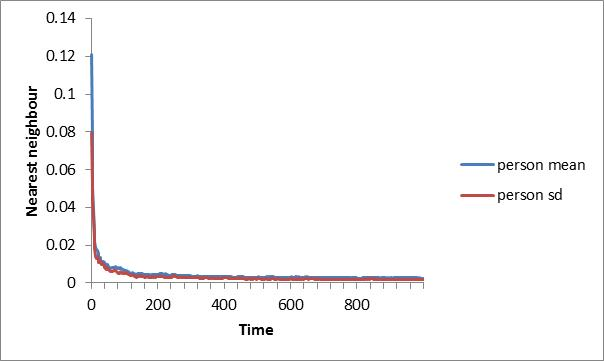
\includegraphics[width=0.4\textwidth]{ChapterFramework/figures/mnnd_blackhole_manyruns1}}
  \hspace{0.2}  
  \subfloat[Firms]{\label{fig:bhg3}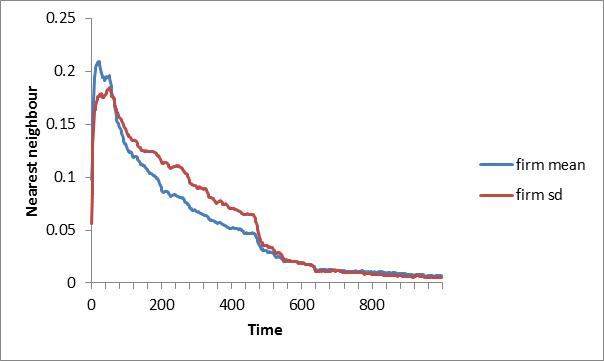
\includegraphics[width=0.4\textwidth]{ChapterFramework/figures/mnnd_blackhole_manyruns2}}
  \caption{Means and standard deviations of nearest neighbour distance, randomised starting locations, averaged from 20 model runs.  \label{fig:blackholegraphs}}
\end{figure}
%Data: location1/data/nearestneigh20runs

Figure \ref{fig:blackholegraphs} shows the outcome of this model run over a thousand days for twenty People and four Firms. The model was run twenty times with different random starting conditions; the data shows the average outcome. All actors converge on a point, incrementally seeking positions closer to each other to reduce space costs or, in Firms' case, increase revenue. People quickly converge, while Firms take much longer: this reflects the fact that Firms must use a feedback that cannot always be relied upon - section \ref{sec:firmsLoV} discusses this point in detail. Ultimately, all actors do reduce their space cost as close to zero as they can.

\subsection{`Monocentric' tests \label{sec:spatialeq}}

%Density cost is used as a proxy to reflect generic `land costs', covering both the effect of rent and congestion (see section x.) 

As discussed in section \ref{sec:densitycostsetup}, a very simple way of avoiding spatial `black holes' where all actors collapse into a point is to impose a density cost. Once again, this is only a partial solution: real land use is subject to the law of supply and demand where actors bid over prices. A density cost can only be a loose proxy. However, it can be used with all the same caveats that attach to any `partial' solution that imposes a fixed cost. This section uses the density cost as a way to test changes in other variables, both spatial and non-spatial, to show the different impact of these. 
 
%The models in this section produce two types of equilibrium result, one that replicates the utility-equilibrium finding from monocentric models, another that breaks it, where Actors' utility does not equilibriate.
%The model setup is the same as for testing the `black hole' outcome above, except for the imposition of a density cost, and an increase in the number of People to a thousand in order to allow a clear picture of the spatial outcome. (Numbers do not directly affect the actual density cost, since it is calibrated to the number of people in any particular model run.)

\subsection{Comparing effect of density cost to black hole outcome \label{sec:densitycomp}}

%%%%%%%%%%%%%%%%%%%%%%%%%%%%%%%
% Scenario table
%%%%%%%%%%%%%%%%%%%%%%%%%%%%%%%
%\input{ChapterModels/Tables/modelatom_firmsLoV_table}
\renewcommand{\arraystretch}{1.2}
\begin{table}[!hbt]
\begin{center}

%\begin{tabular*}{0.8\textwidth}{|l|l|}
\begin{tabular}{|l|l|}
\hline 
\textbf{Component} & \textbf{Description}\\
\hline
Run type & Single run, 1200 days  \\
\hline
Actor type & People $ = 1000$, One Firm \\
\hline
Actor action & Person: optimise utility and position\\
& Firm: static, fixed, all demand met\\
\hline
Space-type & $R^2$\\
\hline
Actor location & People mobile\\
& Single Firm fixed at centre to make `monocentric'\\ 
\hline
Space costs & Iceberg delivery costs for goods \\
& Density cost\\
\hline
Parameters & All fixed except good delivery cost\\
& Good delivery cost changed in discrete values exogenously\\
\hline
Utility form & Single Firm: utility = amount of good\\
\hline
Production form & None: demand always met\\
\hline

\end{tabular}

\caption{Model components for `comparing effect of density cost' \label{tab:cfdensity}}
\end{center}
\end{table}

What impact does a density cost have on model outcome? To test this, the setup from the `black hole' model is used, with two changes. First, Firm location is fixed at a centre-point. Since the feature of interest is density cost, it is assumed that firms have found their way to a central point as they do in section \ref{sec:blackholemodel} above. (Note that, while in the `black hole' model test, Firms do not quite centre perfectly, this small difference from exact centring has no material impact on the test here, so it is easier to assume that centring has taken place.) Second, the number of People is increased in order to allow a clear picture of the spatial outcome.

A test model was run for 1200 days with 1000 People. Over that run, the good delivery cost was exogenously changed twenty-three times, to values ranging from 500 to 0.01. These values were chosen specifically to illustrate discrete changes in the spatial outcome. The visual result for six of these are shown in figure \ref{fig:densityCostChange1}. Green squares are People, grey circles indicate the density cost radius for each Person (see section \ref{sec:densitycostsetup}). The model starts from something close to the `black hole' model where good space-costs are high enough to make density cost relatively unimportant. As good space-costs drop, People self-organise into concentric rings initially, before costs decrease enough for them to find interstitial points that minimise density costs, resulting in the hexagonal pattern observed. This is the result of People trading off density cost against distance to the central Firm.

\begin{figure}[h!]
  \centering
  \subfloat[500]  {\label{fig:dc1}
\includegraphics[width=0.3\textwidth]{ChapterFramework/figures/densitycost1/sequence/torus-0026_FirmDelCost-500}}
  \hspace{0.1}    \subfloat[5]{\label{fig:dc2}
\includegraphics[width=0.3\textwidth]{ChapterFramework/figures/densitycost1/sequence/torus-0301_FirmDelCost-5}}
  \hspace{0.1}    \subfloat[1]{\label{fig:dc3}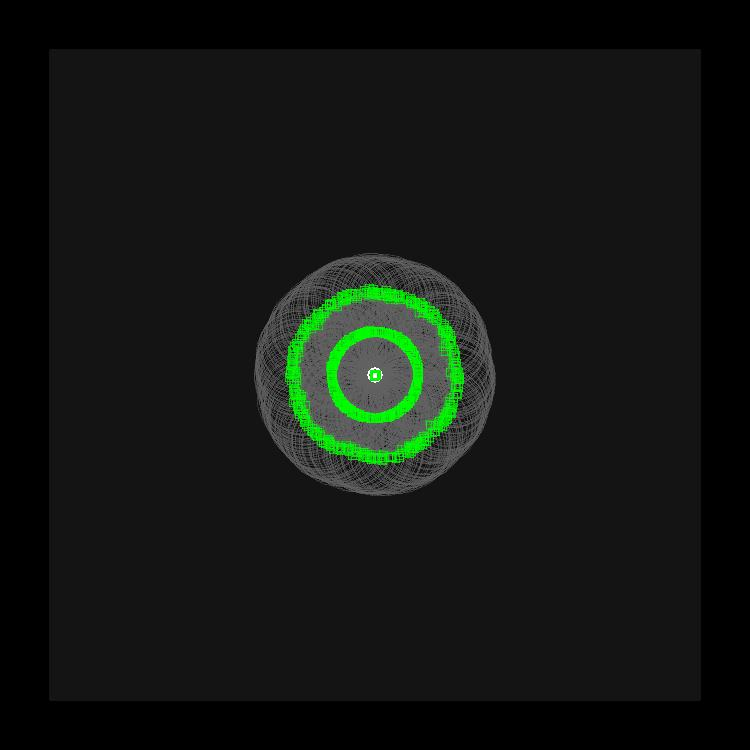
\includegraphics[width=0.3\textwidth]{ChapterFramework/figures/densitycost1/sequence/torus-0376_FirmDelCost-1}}
  \hspace{0.1}    \subfloat[0.5]{\label{fig:dc4}
\includegraphics[width=0.3\textwidth]{ChapterFramework/figures/densitycost1/sequence/torus-0426_FirmDelCost-0-5}}
  \hspace{0.1}     \subfloat[0.125]{\label{fig:dc5}
\includegraphics[width=0.3\textwidth]{ChapterFramework/figures/densitycost1/sequence/torus-0476_FirmDelCost-0-125}}
  \hspace{0.1}     \subfloat[0.05]{\label{fig:dc6}
\includegraphics[width=0.3\textwidth]{ChapterFramework/figures/densitycost1/sequence/torus-0526_FirmDelCost-0-05}}
  \caption{Spatial equilibrium test. Visualisation of good space-cost changes interacting with density cost for six good space-cost values; spatial equilibrium outcome. 1200 days, 1000 People.  \label{fig:densityCostChange1}}
\end{figure}

Figures \ref{fig:dc_util1} and \ref{fig:dc_util2} show the correlation between mean utility versus delivery cost and mean distance from the centre-point versus delivery cost. The morphological outcome - the size of the spread around the centre-point - does not change at the same rate as utility. Figure \ref{fig:dc_util3} gives an indication why: it shows that density cost incurred for each Actor at a given equilibrium point are higher towards the centre. Actors make trade-offs between delivery and density cost, and the impact on utility from changing delivery costs is felt before Actors find new location choices are better. This dynamic is explored in more depth in the following sections. 


\begin{figure}[h!]
\centering
\subfloat[]
{\label{fig:dc_util1}\includegraphics[width=0.4\columnwidth]{ChapterModels/Figures/dc_utilgraph}}%
\hspace{0.2}  
\subfloat[]{\label{fig:dc_util2}\includegraphics[width=0.4\textwidth]{ChapterModels/Figures/dc_mdfcgraph}}
\caption{Spatial equilibrium test. Utility and mean distance from centre versus delivery cost. \label{fig:spatialeq2}}%
\end{figure}


\begin{figure}[h!]
\centering
\subfloat[]
{\label{fig:dc_util3}\includegraphics[width=0.4\columnwidth]{ChapterModels/Figures/DensityCostversusDistanceFromCentrepsd}}%
%\hspace{0.2}  
%\subfloat[]{\label{fig:dc_util2}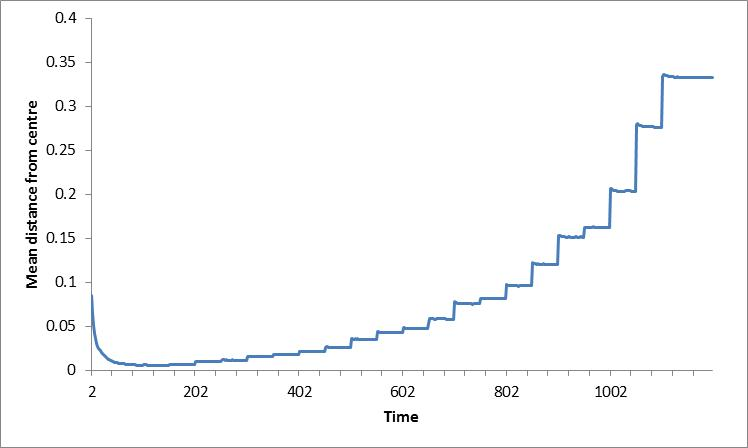
\includegraphics[width=0.4\textwidth]{ChapterFramework/figures/densitycost1/densityseq_meandistfromcentre}}
\caption{At spatial equilibrium, density cost versus distance from centre. \label{fig:spatialeq3}}%
\end{figure}

%Low values for density cost overall, but there we have it. Of course, we knew this: it's a necessary condition for the spatial equilibrium to work. In fact, it's the whole point that (I think) is emerging: the agents are very good at managing to equilibriate, and they'll do that pretty much regardless of how you set the values.
%This begs the question: why and how do they end up with the same level of utility? A fuller exploration of this question is discussed next; a descriptive answer will help set the context for that. 

\subsection{Spatial equilibrium, not utility equilibrium \label{sec:spatnotutileq}}

Initial model runs for density cost tests had very low standard deviation for utility levels across People. It appeared that utility levels were equilibriating - replicating the classic urban economic assumption that $\delta u/\delta d = 0$ as one moves from $d=0$ at the centrepoint to the edge. However, that is not the case in these models: Actors are not always able to find a way to equilibriate utility. They \emph{do} end up in spatial equilibria where no Actor can find a better place to move but, as figure \ref{fig:DC_vs_utilSD} shows, utility levels may differ markedly between Actors. If utility were equilibriating, one would expect its standard deviation to be zero. In some cases, this is so. However, in the example in figure \ref{fig:DC_vs_utilSD}, increasing density cost creates unequal utility levels. 

\begin{figure}[h!]
  \centering  \subfloat[Visualisation, density cost = 250]{\label{fig:dcvusd2}\includegraphics[height=50mm]{ChapterModels/Figures/DensityCost250_unevenutility}}
  \hspace{0.1}    
  \subfloat[Utility S.D vs density cost]{\label{fig:dcvusd2}\includegraphics[height=50mm]{ChapterModels/Figures/DensityCost_vs_UtilSD}}
  \caption{Density cost versus standard deviation of utility, showing that utility moves away from equilibrium.  Height = utility; green = lower utility, red = higher utility. \label{fig:DC_vs_utilSD}}
\end{figure}

Why this outcome? The next sections examine the trade-offs taking place, but here is a quick outline. In the model framework, People do only one thing: compare a range of options and choose the one that makes them better off. In moving, they are not aiming to improve matters for those in denser regions, but that is nevertheless what happens. They reduce density cost both for themselves and for others - but only when doing so allows them to be better off. The flipside is that they will only find moving makes them better off when their current density cost becomes too high, compared to other locations. 

This is, of course, a long way of saying that the system equilibriates. The value of the model is in confirming that this result is an inescapable consequence of many Actors pursuing their own interests - but it also suggests spatial equilibria may not be utility equilibria. There is path dependence: Actors who manage to acquire superior positions find it is not in their interests to change them. Or rather, what happens is that one Actor - when asked to act - finds it best to move further out, lowering density cost for others and relieving them of the need to make that move themselves. As discussed below, this is not a game-theoretic result: the actor that moves faces a static world and makes an optimising decision based purely on that. They are not able to surmise that another actor would be forced to move later, and so wait. And indeed - as discussed in section \ref{sec:nutsnbolts} - if they were, the model would be unable to progress past a synchronous lock-in where no Actor's decision could resolve itself without others doing so first. The following sections look at the trade-offs taking place in more detail.

\subsection{Spatial versus non-spatial cost changes \label{sec:spatvsnon}}

%%%%%%%%%%%%%%%%%%%%%%%%%%%%%%%
% Scenario table
%%%%%%%%%%%%%%%%%%%%%%%%%%%%%%%
%\input{ChapterModels/Tables/modelatom_firmsLoV_table}
\renewcommand{\arraystretch}{1.2}
\begin{table}[!hbt]
\begin{center}

%\begin{tabular*}{0.8\textwidth}{|l|l|}
\begin{tabular}{|l|l|}
\hline 
\textbf{Component} & \textbf{Description}\\
\hline
Run type & Single run, variables correlated \\
\hline
Actor type & People $ = 400$, One Firm \\
\hline
Actor action & Person: optimise utility and position\\
& Firm: static, fixed, all demand met\\
\hline
Space-type & $R^2$\\
\hline
Actor location & People mobile\\
& Single Firm fixed at centre to make `monocentric'\\ 
\hline
Space costs & Iceberg delivery costs for goods \\
& Wage-distance cost\\
& Density cost\\
\hline
Parameters & Each varied, correlated\\
\hline
Utility form & Single Firm: utility = amount of good\\
\hline
Production form & None: demand always met\\
\hline

\end{tabular}

\caption{Model components for `spatial versus non-spatial cost changes' \label{tab:spatialvsnon}}
\end{center}
\end{table}



%%%%%%%%%%

\begin{figure}[h!]
  \centering
  \subfloat[MDFC vs wage]{\label{fig:MDFC1}\includegraphics[width=0.4\textwidth]{ChapterModels/Figures/MDFC_vs_wage}}
  \hspace{0.1}    
  \subfloat[MDFC vs good cost]{\label{fig:MDFC2}\includegraphics[width=0.4\textwidth]{ChapterModels/Figures/MDFC_vs_goodcost}}
  \hspace{0.1}    
  \subfloat[MDFC vs $tech$]{\label{fig:MDFC3}\includegraphics[width=0.4\textwidth]{ChapterModels/Figures/MDFC_vs_tech}}
  \hspace{0.1}    
  \subfloat[MDFC vs delivery cost $c$]{\label{fig:MDFC4}\includegraphics[width=0.4\textwidth]{ChapterModels/Figures/MDFC_vs_dc}}
  \caption{Mean distance from centre Firm (MDFC) for 400 People. Density cost is one, four variables changed. \ref{fig:MDFC1} and \ref{fig:MDFC2} are non-spatial costs, \ref{fig:MDFC3} and \ref{fig:MDFC4} are both spatial costs.  \label{fig:MDFC}}
\end{figure}

Section \ref{sec:reframingpeoplecost} explained that the cost of moving both people and goods can be broken down into spatial and non-spatial cost components. It was through examining the effect of cost changes in this spatial equilibrium setting that this distinction became clear. Initially, the commute time to get to work was built in as part of the wage function, wage being inversely related to distance, as described in section \ref{sec:wageselect}. Testing revealed, however, that changing the spatial component of the wage actually has a different, opposite impact on Actor choices from the wage itself, in exactly the same way that good price has a different impact from its distance cost. In terms of how Actors optimise utility in a setting where density costs are present, it is easier to understand all space costs as equivalent. Thus, a wage can be described in different terms as the price paid in time to buy money or goods directly (This was shown mathematically in section \ref{sec:reframingpeoplecost}).

Figure \ref{fig:MDFC} shows these outcomes for the same spatial equilibrium setup. Here, there is one Firm at the centre, and 400 People buying the Firm's single good. The set of variables are good cost, delivery cost, density cost and tech level. In these tests, each of those four is changed from zero to some higher value (see x-axis in figures) to see the impact on spatial morphology. This is measured using the mean distance of all People from the centre firm, which is larger as People spread further out from the centre. 
%The set of variables are a good cost of 1, density cost of 1, delivery cost of 0.5 and tech level of 1. I

Sub-figures \ref{fig:MDFC1} and \ref{fig:MDFC2} are non-spatial costs. Changing both the wage and the good cost effectively alter the real wage, and both have a spatial impact due to their interaction with delivery and density costs. Increasing the real wage makes People more able to offset density costs and reduce distance cost: they agglomerate. Conversely, $tech$ and $c$ are spatial to begin with, changing the cost of moving goods and wage across space. Decreasing delivery cost and increasing $tech$ have the same effect: goods and wages can get further for cheaper. While overall this increases Peoples' real wages, the spatial effect is opposite: they disperse. 

Model population size does not directly affect the actual density cost, since it is calibrated to the number of people in any particular model run, but number and density cost do interact when there are hard spatial limits imposed.

As mentioned, the method of wage determination combined the wage and distance effects into one: the wage reduces over distance as People have less time to put into Firms. This distance effect for the wage can be turned on or off, so that a change in wage is the same for all People regardless of distance to their chosen employer. If the wage-distance cost is on, however, it does impose a hard limit on People's choices: beyond that limit, no wage is available. As a consequence of having to stay within that limit, if density costs become too high, they simply cannot afford any utility. This is illustrated in figure \ref{fig:UtilityVsDFC_wagedistancecost}, where density cost is high enough to completely wipe out some People's ability to gain utility, while some succeed by reducing the density costs at the edge - an option not open to all because of the hard space cost limit.

\begin{figure}[h!]
  \centering  \subfloat[Visualisation]{\label{fig:uvd1}\includegraphics[height=40mm]{ChapterModels/Figures/DensityCost250w_wagedistanceon}}
  \hspace{0.1}    
  \subfloat[Utility vs distance from centre]{\label{fig:uvd2}\includegraphics[height=40mm]{ChapterModels/Figures/UtilityVsDFC_graph}}
  \caption{Wage-distance on, density cost = 250, few People able to gain utility on edge. White indicates where People are unable to get any utility. \label{fig:UtilityVsDFC_wagedistancecost}}
\end{figure}

\subsection{Understanding the rational choices}

%http://texblog.net/help/latex/ltx-68.html
\renewcommand{\arraystretch}{1.2}
\begin{table}[!hbt]
\begin{center}

\begin{tabular}{|l|l|}
\hline 
\textbf{\large{Region 1}} & \textbf{\large{Region 2}}\\
\hline
\textbf{Both here:} &\\
Wage = 1; no delivery cost; density = 0.5 & \\
Wage - density = 0.5 & \\
G = 0.5; utility = 0.5 each & \\
\hline
\textbf{One here:} & \textbf{One here:}\\
U = 1. No costs at all. & If no delivery or density cost, U = 1\\
& If $U > 0.5$, this region is better\\
& If delivery cost = 1, total good cost = 2.\\
& Wage is still 1, so G = 0.5 = U.\\
& So best to move here if: \\
& $0 < delivery\ cost < 1$\\
& Best to stay in region 1 if:\\
& $delivery\ cost > 1$\\
\hline
\end{tabular}

\caption{Two discrete regions, choice facing two Actors with density and delivery costs: increasing delivery costs is an agglomerating force \label{tab:discretechoicetable1}}
\end{center}
\end{table}

%Table 2, wages

%http://texblog.net/help/latex/ltx-68.html
\renewcommand{\arraystretch}{1.2}
\begin{table}[!hbt]
\begin{center}

\begin{tabular}{|l|l|}
\hline 
\textbf{\large{Region 1}} & \textbf{\large{Region 2}}\\
\hline
\textbf{Both here:} &\\
\textbf{No delivery cost; density = 0.5} & \\
$Wage = 1$ & \\
Wage - density = 0.5 & \\
G = 0.5; utility = 0.5 each & \\
-- & \\
$Wage = 0.75$ & \\
Wage - density = 0.25 & \\
G = 0.25; utility = 0.25 each & \\
-- & \\
\textbf{Wage = 1.25} & \\
Wage - density = 0.75 & \\
G = 0.75; \textbf{utility = 0.75} each & \\
\hline
\textbf{One here:} & \textbf{One here:}\\
No costs at all, so: & \textbf{No density cost, delivery = 1}\\
$U = W = 0.75,\ 1\ or\ 1.25$ & If $wage=1$:\\
& $P_g=2$, $G = 0.5$, $U = 0.5$\\
& --\\
& \textbf{If wage=0.75}: \\
& so $P_g=2$, \textbf{G = 0.75/2 = 0.375 = U}\\
& --\\
& If $wage=1.25$: \\
& so $P_g=2$, $G = 1.25/2 = 0.625 = U$\\
\hline
\end{tabular}

\caption{Two discrete regions, choice facing two Actors with density and delivery costs: three different wages, $0.75$, $1$ and $1.25$\label{tab:discretechoicetable2}}
\end{center}
\end{table}


The following discrete two-region, two-Actor thought experiment helps to reveal the dynamic at work in producing these opposite spatial effects. Consider the following four quantities: wage ($w$), technology ($tech$), good cost ($p_g$) and delivery cost ($c$). $w$ and $p_g$ are both non-space costs: they are not directly affected by distance (though that may be indirectly affected as Actors change prices.) Both $tech$ and $c$ are costs affected by distance. In terms of an Actor's income, increasing the wage has the same effect on their real wage as decreasing good cost: Actors can afford higher density costs and agglomerate accordingly, reducing $d$. Equally, decreasing space costs is real-wage increasing - and yet has the opposite spatial effect in this setting, causing Actors to disperse.

The thought experiment uses the following assumptions. One Firm produces $G$ in region 1, where delivery costs are zero. There are costs to deliver to region 2, however. Two People must decide where to locate to maximise their utility. They can minimise delivery costs by staying in region 1, but if they are both there, density costs are incurred. 

As many variables as possible are normalised: wage and base good price per unit both equal one. Let the density cost be zero if only one Actor is present, and $0.5$ if both are in the same region. If so, subtract the density cost from the wage so it becomes $0.5$ for each Actor. $G$ is the one good, and utility is the same: $G = U$. Delivery cost, in this case, is just one number for the total space cost of moving a unit of $G$ between regions. It could be made up of any mix of distance and per-distance-unit charge.

Tables \ref{tab:discretechoicetable1} and \ref{tab:discretechoicetable2} lay out the options available for the two Actors (excluding both of them choosing to incur both distance and density costs by moving to region 2). The first of these looks at what happens if delivery costs are varied. Increasing delivery cost is an agglomerating force, opposed to the dispersion force of the density cost. If an actor is made to pick the best option available at a given decision point, without reference to what might happen if they wait, they will find moving to region 2 gives them higher utility when delivery costs are between zero and one. Higher than this and they are better off accepting $U=0.5$. Once an actor has moved, it in the interest of neither to change their choice - but if one does move, it allows the other to be better off than them, as it lowers the density cost.

Table \ref{tab:discretechoicetable2} imposes a fixed delivery cost in the second region. It then lays out the utility outcomes for three different wages of $0.75$, $1$ and $1.25$. Looking again from the point of view of a Person picking the highest utility, their best options for each wage are highlighted in bold. If the wage is 1, neither is better: $U=0.5$ in both cases. For the lower wage, region two's $U=0.375$ beats $0.25$ - but note that the Person left behind then gets $U=0.75$. For the higher wage, Region 1's $U=0.75$ beats the further regions $0.625$. In contrast to changes in delivery cost, then, higher wages are an agglomerating force in this scenario. 

In this example, then, the two Actors can end up with differing utility. If many more Actors are introduced, making un-strategic decisions solely based on the best choice from the options presented to them, there is the double effect just mentioned.  They increase their own utility, but also there is a clear externality, as others' utility increases via a lowering of their density cost. This leads to the spatial equilibrium outcome. 

\subsection{Fixing values \label{sec:fixing}}

%%%%%%%%%%%%%%%%%%%%%%%%%%%%%%%
% Scenario table
%%%%%%%%%%%%%%%%%%%%%%%%%%%%%%%
%\input{ChapterModels/Tables/modelatom_firmsLoV_table}
\renewcommand{\arraystretch}{1.2}
\begin{table}[!hbt]
\begin{center}

%\begin{tabular*}{0.8\textwidth}{|l|l|}
\begin{tabular}{|l|l|}
\hline 
\textbf{Component} & \textbf{Description}\\
\hline
Run type & Single run \\
\hline
Actor type & People $ = 400$, four Firms \\
\hline
Actor action & Person: optimise utility and position\\
& Firm: static, fixed, all demand met\\
\hline
Space-type & $R^2$\\
\hline
Actor location & People mobile\\
& Four Firms all fixed at centre to make `monocentric'\\ 
\hline
Space costs & Iceberg delivery costs for goods \\
& Density cost\\
\hline
Parameters & Each Firm has different good cost or delivery cost\\
& Each Person must buy from only one Firm\\
\hline
Utility form & CES (if delivery cost spread)\\
\hline
Production form & None: demand always met\\
\hline

\end{tabular}

\caption{Model components for `fixing values' \label{tab:fixingvalues}}
\end{center}
\end{table}

Other spatial dynamics can be revealed by fixing particular model values. People can be worse or better off relative to each other, depending on cost structure. Real land markets are obviously nothing like as fluid as freely-moving actors: actors unable to respond immediately may display the kind of structure discussed here. Figure \ref{fig:equilfixed} shows a cost-change situation after People's location has been fixed, following a previous period of free movement. If unable to move, increases in density cost can penalise those nearer the centre, or increases in delivery cost can be worse for those on the edge.

\begin{figure}[h!]
\centering
\subfloat[Density cost increased, forms `bowl']
{\label{fig:fixeq1}\includegraphics[width=0.4\textwidth]{ChapterModels/Figures/fixed_eq2crop}}%
\hspace{0.2}  
\subfloat[Delivery cost increased]{\label{ fig:fixeq2}\includegraphics[width=0.4\textwidth]{ChapterModels/Figures/fixed_eq1crop}}
\caption{Post-equilibrium People fixed in position, responding to changes in density and delivery cost. Height = utility; green squares = lower utility, red squares = higher utility. Red lines at ground level are buying lines showing People getting goods from central Firm. \label{fig:equilfixed}}%
\end{figure}

Figures \ref{fig:vonThunen1} and \ref{fig:vonThunen2} fix People to one of four specific Firms. In the first of these, Firms have a range of delivery costs (sub-figure \ref{fig:vt2}). The second has Firms with different good prices (sub-figure \ref{fig:vt2}). In appearance, this is a von-Thunen-like equilibrium, although note the two opposite results again due to whether a spatial or non-spatial variable is changed between Firms. Those People with the lowest costs in both instances do better (marked in red) -  but for delivery costs, the best spatial position is on the edge, while for good cost difference, they locate near the centre.

%Note also that when People are locked in to one Firm's good cost, utility cannot equilibriate, though they are able to improve their utility situation to the extent possible, given density and distance costs. 

\begin{figure}[h!]
\centering
\subfloat[Firm delivery costs]{\label{fig:vt2}\includegraphics[width=0.4\textwidth]{ChapterModels/Figures/vonThunen1_delcosts}}
\hspace{0.2}  
\subfloat[Incurred density costs]{\label{fig:vt2}\includegraphics[width=0.4\textwidth]{ChapterModels/Figures/vonThunen1_densitycost}}
\hspace{0.2}  
\subfloat[Spatial equilibrium]{\label{fig:vt1}\includegraphics[width=0.5\columnwidth]{ChapterModels/Figures/vonThunen4firm}}%
\caption{Four Firms, fixed at a centre point, with a spread of delivery costs. 400 People with density costs optimise location, with each Person `locked' into buying from one Firm only. Matched colours across graphs and visualisation indicate different Firms: in the visualisation, the colour indicates which Firm each Person is locked into. \label{fig:vonThunen1}}%
\end{figure}

\begin{figure}[h!]
\centering
\subfloat[Firm good costs]{\label{fig:vt22}\includegraphics[width=0.4\textwidth]{ChapterModels/Figures/firmCost_vonThunenPrice}}
\hspace{0.2}  
\subfloat[People's utility]{\label{fig:vt33}\includegraphics[width=0.4\textwidth]{ChapterModels/Figures/Util_vonThunenPrice}}
\hspace{0.2}  
\subfloat[Spatial equilibrium]{\label{fig:vt11}\includegraphics[width=0.5\columnwidth]{ChapterModels/Figures/vonThunenPrice1}}%
\caption{Four Firms, fixed at a centre point, with a spread of good costs up to 3.6. 400 People with density costs optimise location, with each Person `locked' into buying from one Firm only. Matched colours across graphs and visualisation indicate different Firms: in the visualisation, the colour indicates which Firm each Person is locked into. \label{fig:vonThunen2}}%
\end{figure}


%Depends on comparable utility... but then, doesn't all urban econs?
%The spatial equilbrium dynamic is able to produce a similar result to the classic von Thunen finding. 
%People are trading off two space costs: density and the cost of moving goods. For these model runs, the former is fixed. When good movement costs change, utility \emph{does} change, and for a period of time, it will vary - but People will self-organise their way back to an equilibrium of utility values. This is the situation illustrated in figures \ref{fig:dc1} to \ref{fig:dc6}. But is it possible to use the model to say more about the nature of this process? 
%It is somewhat surprising that the density cost method produces a spatial equilibrium outcome. After all, no land rent mechanism is present - it is purely a weighted density cost of the sort used in kernel density calculations. So what can account for this? 
%And is it actually as surprising as all that?
%I want to end by confirming that this weighted density cost is (for the purposes here) a reasonable enough proxy for land rent costs that can produce good economic outcomes, without having to directly model land actors and landlords, as I was doing. 
%Also concluding: given some variable land cost, actors will generally equilibriate their utility. That said, of course, I haven't explained why that doesn't happen in backyard yet.
%What all this means: Actors in a spatial equilibrium setting will produce an equilibriated `indifference map' showing where utility is equalised. This is an interactive process, distinct from a purely statistical outcome. A way to illustrate this is to move the two firms apart slightly. Since People have \gls{lov}, what will the `indifference map' look like?
%Actors' ability to collectively produce a spatial equilibrium appears to be independent of the exact nature of the land cost involved. While different methods do produce different spatial morphologies, utility still equilibrates. Figure x compares three visualisations for three slightly different density cost calculating methods.
%This was the realisation I worked through and found:
%MM: That \emph{is} an important element, then: it's the wage itself, not the space cost part of the wage. Higher wages mean you can afford higher density costs, full stop. Now, if the wage distance cost is turned off, that means without a good space cost, actors can located themselves anywhere: space doesn't matter, except to reduce density costs, so they spread out until either the density cost is completely zero, or as low as they can manage given that I keep them within the square.
%MM: It's true that as dc -> 0, you end up with density cost as the only consideration: that is obviously a dispersing force.
%MM: So: the first thing to consider with wages - it's an interaction of three elements, not two. Using the wage-time trade-off confused that: changing the wage with timecost present has exactly the same effect as for delivery cost. (I just checked!) Both reduce real wage over distance (the number of units of good I can get with my wage.)

\section{Moving towards more connected models}

Producing partial models is a relatively straightforward task compared to getting Actors to fully coordinate economic activity. Of the various approaches attempted within this research, many were not able to recreate stable outcomes. Here are three quick examples. One: if the goal is to connect People's labour to production, and thus to stock levels, but also to let Firms set good and wage prices, it is very difficult to get sensible stock levels. Section \ref{sec:prodtowelfare} presents a model that solves this stock problem, but it does it by forcing Actors to target a net-zero stock level. Firms using price-setting behaviour have a hard time producing stable economic outcomes: stock tends either to crash to zero or to increase indefinitely, without prices finding an efficient stock level. Section \ref{sec:firmsLoV} presents a model designed to examine a key aspect of this problem: how Firms use the information they get to set their prices and how they can get it wrong.

Second, the problem of price signalling is thorny. The simple random money flow model in section \ref{sec:comm_costs} demonstrated a key part of the problem: treating money literally as a rivalrous good hits up against the tendency for the flow among many agents to `random walk' into an uneven distribution. The model result even with Actors making more sophisticated maximising choices is that some Firms can end up with the entire money supply - more than they need - while others find themselves in the catch-22 of not being able to pay the wages to produce stock to sell to get money to pay wages. Any economic agent model faces being stuck between this na\"{\i}ve approach to money and finding some other method capable of signalling between Actors. The approach of section \ref{sec:lovprodsetup} is to cut out on layer of complexity by making Actors exchange `input' (like their time) for productive output directly, where the price for the latter is the former. This avoids the need for an intermediary to signal price. 

Lastly, it is also difficult to find any compromise position between partial and general models. For instance, Firms can be given unlimited stock to attempt to avoid the stock problems just discussed. A scenario using the Engel function illustrates the broader problem with this: if there is no stock limit, nothing stops Firms from pricing as close to zero as they can. The result is - in the case of the Engel function - luxury producers can price so low that the model reverts to the Cobb Douglas outcome of the share parameter dictating the split of revenue between sectors. Firms act rationally then - but a world of infinite stock makes a mockery of the idea of luxury and necessity goods. 

Given this, section \ref{sec:prodtowelfare} presents a model that does manage a `general' outcome, in that production is connected efficiently to welfare through price signals, and explains the methods used to do so. The next section examines one particular agent barrier to using price signals to achieve coordination.

\subsection{`Data, meaning, response' with two Firms \label{sec:firmsLoV}}

%%%%%%%%%%%%%%%%%%%%%%%%%%%%%%%
% Scenario table
%%%%%%%%%%%%%%%%%%%%%%%%%%%%%%%
%\input{ChapterModels/Tables/modelatom_firmsLoV_table}
\renewcommand{\arraystretch}{1.2}
\begin{table}[!hbt]
\begin{center}

%\begin{tabular*}{0.8\textwidth}{|l|l|}
\begin{tabular}{|l|l|}
\hline 
\textbf{Component} & \textbf{Description}\\
\hline
Run type & Parameter sweep, changing utility noise levels\\
& and changing random seed\\
& Single model run ends when Firms complete goal, see below.\\
\hline
Actor type & Two Firms, a small circle of People\\
\hline
Actor action & Firms: optimise location only\\
& People: spend set wage only\\
\hline
Timing &
Randomised bloc for each bloc of Firms \& People\\
\hline
Space-type &
$R^2$\\
\hline
Actor location & Firms begin on edge, People fixed in circle\\
\hline
Space costs & Iceberg delivery costs for goods\\
&People pay this cost; Firms only receive good unit price\\
\hline
Parameters & All fixed, except utility noise level\\
\hline
Utility form & CES (love of variety)\\
\hline
Production form & None: demand always met\\
\hline

\end{tabular}

\caption{Model components for `Data, meaning, response' with two Firms' \label{tab:firmsLoV}}
\end{center}
\end{table}

A prerequisite for fully connecting production to welfare is Actors capable of successfully using cost signals to change their behaviour. Section \ref{sec:prodtowelfare} describes a scenario where these signals successfully lead to a higher-welfare outcome. The following example looks at a partial model to illustrate that the problem of cost signalling can be a challenge. Firms make only one decision: where to move? Getting closer to their market should, in theory, increase income - and indeed, if only a single Firm exists, it has no problem finding an income-maximising path. The rest of the world is static, so any change must be a consequence of its own actions. As soon as a second Firm is added, however, that is not the case. Confounding factors then mean they may fail to interpret the meaning of their cost signals correctly. 

This model asks two Firms to play a `game' on both a line and in $R^2$. Firms are placed an equal distance from a circle (or short line) of immobile People who are fixed at the centre within a small radius. The Firms can attempt to improve their revenue only by moving. Their revenue-maximising position is near the centre of the People, where delivery costs are minimised. A game terminates either when both Firms have succeeded in getting inside the radius of the People or ten thousand days has passed. Figure \ref{fig:2firmgamevis} illustrates the endpoint of the game in $R^2$.
%Though the Firms do not receive these delivery costs, anything People do not need to spend on them ends up as extra demand for the goods.

\begin{figure}[h!]
\centering
\subfloat[$\rho=0.995$]{\label{fig:2fg11}\includegraphics[width=0.4\columnwidth]{ChapterModels/Figures/2firmgame_rho_nearly1cropped}}%
\hspace{0.1}  
\subfloat[$\rho=0.5$]{\label{fig:2fg22}\includegraphics[width=0.4\textwidth]{ChapterModels/Figures/2firmgame_rho_halfcropped}}
\caption{Two Firms at `winning' position in centre of circle. Lines indicate buying strength from People: when goods are fully substitutable ($\rho\approx1$) People buy from nearest Firm. When there is love of variety, they buy a mix from both. \label{fig:2firmgamevis}}%
\end{figure}

Firms play an array of these games: utility noise levels are parameter-swept and for each value the random seed is altered a given number of times to then produce an average for all games with that value.

What is the rationale behind this? To put it into \gls{dmr} terms (see section \ref{sec:dmr}) a Firm has only one datum to act on, a change in revenue. The meaning of an increase is taken to be, `my previous action was successful'. Conversely, a drop in revenue is taken to mean that the action was counter-productive. This leads to the subsequent response: either repeat the action or reverse it. The broader meaning for the Firm in this situation is: `my actions can determine my revenue levels'. Problems arise when this meaning is incorrect: a Firm may take an action, but if its revenue levels are not determined solely by that action, there is scope for misinterpretation, and thus a faulty response. 

The aim is to provide a `god's eye view' of the Firms' goal in as simple a cost-signal setting as possible. The optimum they are aiming for is clear. Firms having to get to a central point is, from the modeller's point of view, an entirely objective and clearly defined goal, while at the same time, opaque to the Firms, since their `view' is restricted to revenue data. If they were not forced to use revenue alone to `feel' their way, they could obviously be programmed to head straight for the centre of the circle. This makes it an easier example to consider than attempting to set prices. This combination - a single action, trying to optimise a single value - makes it useful for thinking about the problem. If Firms attempted to optimise other values (price or wage, for example) it would be considerably more opaque.

Although this looks like a Firm location model, it should not be thought of as one. Its purpose is to think about how Firms make decisions given (possibly noisy) information. Even putting aside that firms obviously do not `grope' their way to more productive locations, they would in reality be able to make much more informed location decisions. The problem here is more akin to having to make pricing decisions in a small monopolistic competition situation, where both other firms' and people's actions affect outcomes. The question is: in as simple an example as possible, what gets in the way of a Firm making an appropriate response to correctly interpreted data?

A full description of the setup for the `game' test is as follows. People are set in a stationary circle at the centre of an $R^2$ space, or in a bounded line in $R^1$. Two Firms must find an optimal location that maximises their revenue. All prices and wages are fixed, and Firms' stock is unlimited. Delivery costs are `iceberg': People pay a delivery cost, but it `melts away' and Firms receive just the unit value. This means that, from the point of view of People, cost per unit drops as Firms draw closer. They can then afford to buy more. This means that a Firm's revenue-maximising location (in the absence of any others) is directly in the centre of the circle of people. A Firm's decision process is this:

\begin{itemize}
	\item At time $t-1$: Try a new location near to my current one. If in $R^1$, this will be in one of the two available directions. If $R^2$, it will be a random vector defined by an angle and magnitude (as the magnitude is increased if the guess was successful; see section \ref{sec:howFirmsAct}).
	\item At $t$: did my revenue improve?
	\begin{itemize}
	\item Yes: repeat the previous action, increasing the distance slightly
	\item No: revert to last good location
\end{itemize}
\end{itemize}}

In this example there are five key factors that impact on revenue. The first is a Firm's own actions -just moving to a new spot. The second comes indirectly from the actions of other Firms: they may move to a location that leads People to shift demand to them, and this in turn may make other Firms' revenue-flow negative where it would otherwise have been positive. The other three factors all relate to the connection between People's demand levels and noise. If People are using pure constrained utility - thus providing a crystal-clear demand signal - Firms have no problems making correct decisions about changes in revenue. However, if demand is less clear than this from turn to turn, revenue signals become less reliable. More than this, as noise increases, the value of $\rho$ - the level of \gls{lov} in the model - begins to determine Firms' success rate.

In the model framework, noise naturally appears when using the greedy algorithm, and it is noisier the less iterations are used. As section \ref{sec:optimisingbundles} explained, the algorithm starts by guessing budget slices for all available goods. With fewer iterations, these guesses are further from the `perfect' optimisation, and thus demand fluctuates. It is in running greedy algorithm models that the impact of noise on Firm optimisation becomes apparent. However, for the sake of computational expense and feasibility of large parameter sweeps, a noise term has been added to the constrained utility methods.\footnote{While a noise term can be added to the constrained algorithm, it is quite hard to make it economically sensible. This requires staying in budget: the greedy algorithm does this by design. Adding noise to constrained utility, however, may mean People appearing to spend slightly too much or too little. Avoiding this is actually a large optimisation problem in itself, since there is no way to `read back' from constrained good quantities.} 

The noise term just adds a random fluctuation to the optimal good quantities the constrained algorithm finds. For instance, if $noise=0.5$, the optimal quantity is randomised in a range of plus or minus half its total value.

Firm and Person numbers are the final two factors, both impacting on demand noise level, if any is present. Both have a similar effect, for different reasons. Increasing the number of People means a larger source of demand for each Firm's goods, thus tending to average any noise out as these rise. Rather less intuitively, increasing Firm numbers reduces noise when using the greedy algorithm simply because the variance of size of budget slices drops. A budget randomly split between two Firms will have a much higher variance than one split between ten or a hundred. Constrained utility noise is equally lower, as it is applied proportionally to the quantity of optimised good amount.

Figure \ref{fig:FirmGame1} graphs the average number of days it took both Firms to get inside the circle of People, for a range of values of $\rho$ up to 1, in $R^1$. A hundred randomisations were averaged for each value of $\rho$. Three different noise levels were tested: it can be seen that when no noise is present, $\rho$ makes no difference to the success of Firms' decisions. As the noise level increases, however, $\rho$ begins to be important. High levels ($\rho \rightarrow 1$) present no problem, regardless of noise level. However, as \gls{lov} increases ($\rho \rightarrow 0$) noise increasingly interferes in a Firms' ability to correctly identify revenue-improving positions.

\begin{figure}[h!]
\centering
\subfloat[$noise = 0$]{\label{fig:fg11}\includegraphics[width=0.6\columnwidth]{ChapterModels/Figures/FirmGame11}}%
\hspace{0.1}  
\subfloat[$noise = 0.1$]{\label{fig:fg12}\includegraphics[width=0.6\textwidth]{ChapterModels/Figures/FirmGame12}}
\hspace{0.1}  
\subfloat[$noise = 0.5$]{\label{fig:fg13}\includegraphics[width=0.6\textwidth]{ChapterModels/Figures/FirmGame13}}
\caption{Firms compete to reach centre of market. Number of days to success on vertical axis, value of $\rho$ on horizontal. Mean and S.D. for a hundred randomisations of each value point. Three different noise levels. Note for figure \ref{fig:fg13}, days to complete are an order of magnitude higher than for \ref{fig:fg12}. \label{fig:FirmGame1}}%
\end{figure}

The implications of this are discussed in more detail in the final chapter, in the context of the various approaches to coordination taken in the thesis. 

%Now, is this because of $\rho$'s effect on People's choices, or its effect on how Firms' decisions interact with each other?
%In contrast to objective optima possible in analytic approaches, in this situation Firms cannot know whether their current revenue has reached a point of final optimum. In practice this means they will always need to `test the waters' looking for further improvements. A consequence of this is that they may cede revenue, and leave a space for others to exploit. No one Firm can act without changing the situation others face. Attempting to seek revenue improvements thus becomes a constant battle, unable ever to stabilise.
%There is, however, a region of stability within which this battle for revenue takes place, and once a Firm has found it, they able to hold that position.
%Note that Firms test only for an increase in sales since the last turn. Outgoing costs do not enter into the calculation: wages are fixed, and so it makes no sense for Firms to have to pay them.


\section{The `transmission belt' between production and welfare \label{sec:prodtowelfare}}

In this section, a single-actor model is presented that succeeds in linking production to welfare levels. It builds on concepts developed in the preceding analysis, finding a simple solution that allows efficiencies from economies of scale to feed through to improvements in utility. Actors' \gls{lov} is used as a way to circumvent \gls{bertcomp}-like problems with wage-setting, where a wage offer only minutely higher than others will automatically be selected. Actors also receive their wage directly in the form of goods, so as to avoid any complicating currency issues. The full description of the set-up is in section \ref{sec:lovprodsetup}

Before that, section \ref{sec:singleActorLoVAnalytic} spends a little time demonstrating that, analytically, it is possible for two productive actors to trade across a distance with only one of the two types of \gls{increts}. \gls{lov} alone can be enough of an incentive. Note that it does not preclude the black hole condition: actors would still prefer to minimise space costs. This is done to demonstrate that single-actor-type trade across space, with onlly \gls{lov}, is at least theoretically feasible.

\subsection{Single actors breaking out of their backyards \label{sec:singleActorLoVAnalytic}}

What are the minimal conditions needed to persuade actors to trade, if they are able to produce in their own `backyard?' As discussed in section \ref{sec:marketstructure}, \gls{increts} are a necessary (but not sufficient) condition. Those \gls{increts} do not need to come from a Firm's economies of scale, however. Love of variety alone, with linear output, is enough to make it worth actors' time to move out of their backyards and trade. This section presents a short analytic example illustrating how it is possible for two actors with \gls{lov} alone to prefer trade.

%Table \ref{tab:spatimpsimple} lists the model component settings. As described, two types are compared here to illustrate their equivalence: one where \gls{increts} come from love of variety alone, and one with production-level \gls{increts}.

%%%%%%%%%%%%%%
% Scenario table
%%%%%%%%%%%%%%
%\input{ChapterModels/Tables/modelatom_increts_table}

The situation is this:

\begin{itemize}
	\item Two actors $A$ and $B$, a given distance $d$ apart.
	\item Each produces a unique good ($A$ makes $F$ and $B$ makes $M$) in their backyard using time. Time can also be used to move across space. Let any distance travelled by $A$ and $B$ equal $d_A$ and $d_B$. Let any time put into labour equal $l_A$ and $l_B$ respectively. Production is linear (and normalised to one) so $F = l_A$ and $M = l_B$. Each actor's `budget' is one day - so for example, for actor $A$, $d_A + l_A = 1$. (So movement cost is also linear, e.g. $d_A = 1 - 1_A$.)
	\item Both actors have a pure-good \gls{ces} utility function of the form already described in equation \eqref{eq:-4}: $U = (F^\rho + G^\rho)^{1/\rho}$. This means that if they consume only the good they make (the backyard scenario) utility is proportional to good production, since e.g. $U=(F^\rho)^{1/\rho} = F$.
\end{itemize}

Trading is worthwhile only if it gives actors higher utility than backyard production: a simple comparative statics problem. (The next few paragraphs will describe the situation for actor $A$ to save repetition.) In the normalised example above, backyard production just gives $U = F = 1$. That is, utility is always proportional to the good quantity produced, and the amount produced is always just proportional to the time put in (for backyard production, $l_A = 1$ since there is no movement). 

So trade will be better than backyard production if $U > 1$ for both actors. To help work out when this is true, some assumptions can be used from what has already been shown in section \ref{sec:CESbasics} and more formally in appendix \ref{apx:maths}. \emph{If} trade does take place, the optimal mix of two goods is a perfectly even split, $F=G$. Given what has just been stated about space costs, this means there is one unique location that will optimise utility from trade, if it is to take place at all: exactly half-way between the two actors, at $d/2$. (Note also, if they were delivering goods to each other, rather than meeting in the middle, this would by itself guarantee an even split, since $d_{AB} = d_{BA}$.)

Trade can only occur if anything has actually been produced. Total production for the two actors, $F+M$, is zero-sum with distance. It is straightforward to show that total good production in trade is $F+M = 2-d$ - that is, if the total distance between them is more than two, nothing will be produced. This gives a maximum distance beyond which no trade can take place. Now, given the assumption that a trading optimum is an even split, each actor's optimum is just half the total: $F+M = (2-d)/2$ or $1-(d/2)$. This quantity can stand in as a budget constraint for each agent. Using it to optimise \eqref{eq:-4} produces similar results to that outlined in the appendix. $F=M$, but the optimal quantities of each in relation to distance are slightly different: $F=(2-d)/4$ and $M=(2-d)/4$.\footnote{To check this, only the partial equation for $dZ/d\lambda$ needs changing from that outlined in section \ref{sec:constrainedopt}. This is just the budget constraint described above, which $F=M$ can be plugged into to get quantities for $F$ and $M$.}

\begin{figure}[h!]
\centering
\includegraphics[width=0.85\columnwidth]{ChapterModels/Figures/CESTwoPartnertradeGraph}%
\caption{Two-actor CES, backyard or trade? Love of variety ($\rho$) on the y axis, total distance ($d$) between actors on the x axis. Thick red line indicates where $U=1$: this marks the break between `backyard or trade'. Blue line, $U=1.2$ and red line, $U=0.8$. \label{fig:CESTwoPartner}}%
\end{figure}

How to find whether trade is actually better than backyard alone? Given that this happens only where trade gives $U>1$, an easy option is to start by identifying where $U=1$. This can give a line separating trade from backyard. The fact that we already know there will be an even mix makes this easier: the optimal quantities for $F$ and $M$ can just be plugged into the utility function. Given that both quantites are the same -

\begin{equation}
U = (2\cdot(\frac{2-d}{4})^\rho)^{1/\rho}
\end{equation}

Isolating for $d$ gives: 

\begin{equation}
%d = -4(\frac{1}{2}U^\rho)^{1/\rho}+2
d = -4(U\cdot2^{-1/\rho})+2
\end{equation}

That is, plugging any target utility value in for $U$ and $\rho$ gives a distance line for that utility. Figure \ref{fig:CESTwoPartner} shows three lines, indicating where trading gives better utility than sticking to backyard production. Where $\rho=1$, and the two goods are perfect substitutes, both actors would need to occupy the same point in space: this would be no different to producing for themselves. The further apart they are, more love of variety is required to make up for the distance cost - until distance itself rules out production altogether.

This example shows that, even with a hard spatial limit and without actual economies of scale, it is possible to actors to have an incentive to trade. The model presented next introduces an addition to these assumptions by allowing Actors to use a \gls{ces} function with no hard limit, so they can optimise their choices - including their own produced good. But it also introduces economies of scale at the production level. The question then becomes, can the Actors find a collective route to efficient, welfare-maximising production?

\subsection{Love-of-variety production-welfare model \label{sec:lovprodsetup}}

%%%%%%%%%%%%%%%%%%%%%%%%%%%%%%%
% Scenario table
%%%%%%%%%%%%%%%%%%%%%%%%%%%%%%%
%\input{ChapterModels/Tables/modelatom_firmsLoV_table}
\renewcommand{\arraystretch}{1.2}
\begin{table}[!hbt]
\begin{center}

%\begin{tabular*}{0.8\textwidth}{|l|l|}
\begin{tabular}{|l|l|}
\hline 
\textbf{Component} & \textbf{Description}\\
\hline
Run type & Single run \\
\hline
Actor type & Single actor type only \\
& People number $=40$ or $80$\\
\hline
Actor action & Optimise utility, position, stock level\\
\hline
Space-type & None or $R^1$\\
\hline
Actor location & Mobile, random starting position\\
\hline
Space costs & Iceberg delivery costs for goods \\
\hline
Parameters & Each Person has `given' exogenous time/input\\
& Each Person is also producer,\\
& has stock level \& good price\\
\hline
Utility form & CES (love of variety)\\
\hline
Production form & smooth economies of scale\\
\hline

\end{tabular}

\caption{Model components for `love-of-variety production-welfare model' \label{tab:lovsingleactor}}
\end{center}
\end{table}


The motivating goal for this model is this: connecting input into production to good output produced through \gls{eos}. Then, getting those goods priced correctly so that welfare is maximised. It is a `proof of principle', showing that production and welfare can be coordinated using these particular methods. 

The setup is a contrast to previous ones, and can be a little confusing since it combines a number of different value concepts. Consider Actors $A$ and $B$. $A$ buys goods from $B$, but the `currency' is a generic input that $B$ then uses in production. Each Actor has a set daily amount of this `input' to spend on goods. It can be considered time: everyone gets a flow of `one day per day' to optimise. Since it is \gls{ces} utility, everyone buys at least a little from everyone else - unless $\rho = 1$, in which case goods are fully substitutable and the cheapest will be favoured. The goods sold can be considered the direct wage paid to $A$ for their input; they are thus able to get this `wage' from many different producers.

While simpler in principle than a Person-Firm model, in this example each Actor actually contains two logically compartmentalised functions, one dealing with consumption, the other production. They both happen in the same object, but are distinct from each other functionally. One part does the buying, maximising utility in the usual way. A \gls{ces} function optimises, on goods sold using the `goods plus delivery cost' equation from section \ref{sec:costmovinggoods}, $P_g = p_g + (c \cdot d)$. Any good-movement costs `melt away'. 
%It is given one unit of input per day to spend; because it can be spent on both moving goods across space and production, it could be considered as time.

The second compartmentalised element in each Actor deals with selling and production. Production has economies of scale: higher input produces a higher per-unit output. The method of achieving this is to use the smooth \gls{eos} function described in section \ref{sec:prodfuncts}. The fixed-cost, \gls{coremodel} style of production function is, in the model as currently set up, unable to produce the desired connection between production and welfare, for the reasons described in section \ref{sec:blindvsrational}. 

Two variables manage the production coordination job in tandem through a feedback: base good price $p$ and stock level $s$. Each actor has one simple goal: keep net stock levels at zero. They are actually programmed to have efficiency as their goal, then: there is no economic motivation for them doing so, though in aggregate all Actors do benefit with higher welfare if this efficiency is achieved. 

There is another consequence of combining the consumption and production functions in one actor: the location decision is made based on the utility decision alone. The geographical point of production thus follows the demand by default, in much the same way it does in the \gls{coremodel}.

The zero target for net stock can be made physically `plausible' simply by assuming actors have stock buffers. Zero then becomes their target production level rather than a physical lower limit. Indeed, the model can be set up to reach a given arbitrary level of production and then work from there, leaving a positive buffer. For the sake of ease of discussion, though, a target of zero is assumed.

Several interconnected problems need solving for this model to work. At the heart of the issue is cost, currency and stock. Implementing any kind of currency system is avoided by allowing the goods themselves to directly be the wage. This is made possible by using the \gls{ces} approach to getting inputs into production, explained in more depth below. Then, stock levels need to avoid two pitfalls. First, for economies of scale in production to feed through to welfare, any efficiency gains needed to actually be consumed. It is no good if stock merely piles  up: the connection would be broken between efficient production and utility. At the other end, the model must avoid `crashing' because no stock exists, and thus no incentive to work or buy is present - the catch-22 situation described in section \ref{sec:blindvsrational}. 
%\cmt{somewhere I have the example of how its possible for Firms to prefer stockpiling.}

The first solution is, as Fowler does (see section \ref{sec:fowler}), to always allow demand to be met. In contrast to the two-timestep feedback decisions of Firms, stock levels are then controlled through ongoing `granular' price adjustments. As mentioned, this does not arise from Actors' maximising behaviour, though it is a `market mechanism' in the sense that price signals are used to achieve the goal. Instead, it is specifically designed to find the efficient level of production. This price adjustment occurs every time an Actor buys. Several things happen simultaneously. If $A$ buys from $B$, let the input from $A$ be $i_A$, the good sold by $B$ be $g_B$, with base price $p_B$. In the model presented here, the process is:

\begin{itemize}

\item $A$ chooses their best Bundle using their unit of input as the budget. Since it is a \gls{ces} function, all Actors will receive some share of this, minus the space cost that `melts away'.

\item $B$ pays with its good $g_B$, and stock is reduced accordingly. 

\item $B$ receives a quantity of input $i_A$ in return, which goes straight into production. The production amount is worked out as described in section \ref{sec:abmprod}: economies of scale come from all input from recent interactions, and the actual productive output is calculated when $A$ buys: it is proportional to the current input from $A$, $i_A$.

\item There is now a net stock level from this one interaction, which $B$ uses to guide their price adjustment. If stock is more than zero, demand was lower than production, and so $p_B$ is lowered to try and sell more. If stock is less than zero, demand was higher than production, and $p_B$ is increased to sell less. 

\item The change in price used is proportional to the amount that stock levels deviate from the target amount: $\triangle p_B = (stock^2)/x$, where $x$ controls the size of the price change. If stock is near its target, then, price changes are smaller. If stock is zero, the price change is also zero.

\end{itemize}


In meeting the zero-stock target, the price signal must balance the two competing effects from changing the price. Reducing it increases demand, but it also increases input into production. That is not unique to this scenario: in any model with a small enough number of Actors, changing price is always in effect changing the real wage. It must, however, find the point where these two balance. It cannot be described in the same way that a Firm would aim for $MC=MR$ (see section \ref{sec:marginalapx}) since the incoming and outgoings units are not the same. 
%I have no idea how that actually ends up producing a working model. Sometimes it doesn't. Interesting.
%check comments at MM: "On the stock price signal [23.8.11]"

Note that the order of Actors added to a Bundle is randomised also. This matters more for this model since, when each Actor buys, they are doing so from every other Actor. 

Figure \ref{fig:eosm} shows a result for a non-spatial run, with eighty Actors. The \gls{eos} `multiplier' does just that: multiplies the function by a given factor. If the model is working, then, utility should be expected to increase linearly with the multiplier, as it does in sub-figure \ref{fig:eosm1}. Note, this is of course an artificial imposition of increases in production, not Actors moving further up the existing \gls{eos} curve themselves by optimising spatial location, but it is an effective test. Sub-figure \ref{fig:eosm2} shows Actors' price-setting behaviour: prices drop overall as production efficiency increases, and they find a new point of net zero stock that can take advantage of it.

\begin{figure}[h!]
\centering
\subfloat[EoS multiplier vs mean utility]{\label{fig:eosm1}\includegraphics[width=0.4\textwidth]{ChapterModels/Figures/EoSmulti1}}
\hspace{0.1}  
\subfloat[EoS multiplier vs mean price]{\label{fig:eosm2}\includegraphics[width=0.4\textwidth]{ChapterModels/Figures/EoSmulti2}}
\caption{Economies of scale `multiplier' versus mean utility and good price set by all actors. \label{fig:eosm}}%
\end{figure}

Figure \ref{fig:eosmpic1} shows two outputs of utility levels for all Actors for 500 days. In sub-figure \ref{fig:eosm3}, the \gls{eos} multiplier is increased at regular intervals. While Actors do find optima, the first change causes some difficulty for the system as a whole. This is a common feature of the method as it stands: many Actors attempting to equilibriate their stock levels via price can produce complex internal dynamics that do not always succeed in stabilising. Sub-figure \ref{fig:eosm4} shows one such situation, where the multiplier is very low. Utility levels stay bounded, but they do not settle. Note that all Actors follow the same oscillation (their utility levels all overlap into one thick line).

\begin{figure}[h!]
\centering
\subfloat[EoS multiplier vs utility over model time]{\label{fig:eosm3}\includegraphics[width=0.7\textwidth]{ChapterModels/Figures/EoSutil2copy}}
\hspace{0.1}  
\subfloat[EoS multiplier vs utility]{\label{fig:eosm4}\includegraphics[width=0.7\textwidth]{ChapterModels/Figures/EoSutil1}}
\caption{Economies of scale `multiplier' versus utility, showing (\ref{fig:eosm3}) response to changes in the EoS `multiplier' and (\ref{fig:eosm3}) failure to break out of internal oscillation dynamic. \label{fig:eosmpic1}}%
\end{figure}

While Actors do succeed in connecting productive efficiency to welfare, then, it is not always smooth, as feedbacks in their attempts to equilibriate stock can produce erratic behaviour. Nevertheless, they are able to make the connection between production and welfare, and there is scope for testing further methods of coordination. 

\subsection{Space, love of variety and economies of scale \label{sec:loveos}}

This section looks at an outcome from the above model showing the interaction between space, \gls{eos} and \gls{lov}. Actors are fixed at even intervals along a line of unit length. Delivery cost is set to ten: this is the only space cost. As section \ref{sec:cesspace} explained, once a distance cost has introduced heterogeneity into total good cost, then changes in the value of $\rho$ will have spatial effects. The consequence in this single actor scenario is that as $\rho\rightarrow1$ and goods become more substitutable, Actors are able to find a route to better utility through a change in production structure. 

It is also the case that, for a certain range of $\rho$ values, changing the delivery cost will affect production stucture. For higher values of $\rho$, where goods are more substitutable, lower delivery costs make it more feasible for single producers to dominate: they can produce more efficiently while delivering the output further.
 
The dynamic is a result of an interaction between two model elements: price-changes to meet the  net zero stock target and demand shifts as overall good costs change. Actors are not only able to discover equilibria, but they can find a route between them.  In the case where $\rho\rightarrow1$, for example, higher demand for single varieties means a feedback between increasing efficiency and lower price for single producers. 

Figures \ref{fig:transspace1} and \ref{fig:transspaceEoS1} illustrate the model for 40 Actors. The first of these shows a visualisation of the endpoint of the model run and a graph of the process to get there. In sub-figure \ref{fig:transvis}, height of squares show the amount of contributed input going into each actor from others: those with the highest have emerged as the main sites of production. Sub-figure \ref{fig:transgraph} graphs the same value: contributed input. Over the run, it is possible to see how some emerge as main producers and others lose input.

\begin{figure}[h!]
\centering
\subfloat[Visualisation: height of coloured squares = contributed time]{\label{fig:transvis}\includegraphics[width=0.8\textwidth]{ChapterModels/Figures/transitionContTimeVizCropped}}
\hspace{0.1}  
\subfloat[Graph: contributed time]{\label{fig:transgraph}\includegraphics[width=0.8\textwidth]{ChapterModels/Figures/transitionContTimeGraph}}
\caption{Actors fixed at even intervals along a unit line, delivery costs = 10. Contributed time change as rho moves from 0.5 to 0.9. Visualisation shows end of this process, with a few large producers emerging. \label{fig:transspace1}}%
\end{figure}

Figure \ref{fig:transspaceEoS1} indicate which percentage of Actors received more than 1.5 units of input as the values of $\rho$ (\ref{fig:transrho}) and delivery cost (\ref{fig:transdel}) change. In sub-figure \ref{fig:transrho}, delivery costs are fixed to 10. As $\rho\rightarrow 1$ and goods become more substitutable, the percentage of higher-output producers increases. Keeping delivery costs fixed, however, means that less centralised production can emerge than is the case in sub-figure \ref{fig:transspaceEoS1}. Here, $\rho$ is fixed at 0.85 and delivery costs are changed. There is a double effect: as delivery costs drop, more input becomes available overall since less is `melting away' on moving goods across space.This increase in total input initially dominates, with a similar effect to increasing $\rho$: the total number of larger producers increases. However, as delivery costs decrease further, the number of large producers goes down to two (5\% of 40): the very low delivery costs allow for a small number of very efficient producers to `deliver' far away.

\begin{figure}[h!]
\centering
\subfloat[$\rho$ vs input, holding delivery cost at 10]{\label{fig:transrho}\includegraphics[width=0.4\textwidth]{ChapterModels/Figures/rhovsinput}}
\hspace{0.1}  
\subfloat[Delivery cost vs input, holding $\rho$ at 0.85]{\label{fig:transdel}\includegraphics[width=0.4\textwidth]{ChapterModels/Figures/delcostvsinput}}
\caption{Change in the number of actors receiving more than 1.5 units of contributed input, for changes in $\rho$ (\ref{fig:transrho}) and delivery cost (\ref{fig:transdel}). \label{fig:transspaceEoS1}}%
\end{figure}

A question that arises from the above: is it actually the case that Actors are making welfare-maximising choices when they move between spread-out and centralised production? That is, does utility increase overall? Figure \ref{fig:transrhographvis} indicates what happens with 10 Actors fixed over a line. From an even mix of production (or nearly, given those on each end will receive less) one central producer emerges as $\rho \approx 0.76$. As can be seen, this is a utility-maximising choice overall. As would be expected, utility decreases as \gls{lov} drops. At a certain point, however, Actors find a path to a higher-utility equilibrium, investing their time into one producer. This is seen from the `kink' in average utility in sub-figure \ref{fig:transrhoutilchange1}. Note, however, the spread of utility for all Actors in sub-figure \ref{fig:transrhoutilchange2}: those closer to the single centralised producer do better than others. 

\begin{figure}[h!]
\centering
\subfloat[Input per Actor: production spread out]{\label{fig:transrhoutilchangexx}\includegraphics[width=0.9\textwidth]{ChapterModels/Figures/EoSrho2}}
\hspace{0.1}
\subfloat[Input per actor: single producer]{\label{fig:transrhoutilchangeyy}\includegraphics[width=0.9\textwidth]{ChapterModels/Figures/EoSrho1}}
\hspace{0.1}
\subfloat[Correlation: $\rho$ vs mean utility]{\label{fig:transrhoutilchange1}\includegraphics[height=35mm]{ChapterModels/Figures/utilityrhocorrelation}}
\hspace{0.1}  
\subfloat[All Actors' utility over model time as $\rho$ increases]{\label{fig:transrhoutilchange2}\includegraphics[height=35mm]{ChapterModels/Figures/RhoTransmissionUtilChange2}}
\caption{10 Actors, delivery cost = 1. Mean utility versus $\rho$ and all Actors' utility as $\rho$ is changed in model time. The `kink' in utility indicates where Actors transition to a single central producer. \label{fig:transrhographvis}}%
\end{figure}




%===========
\begin{comment}
..
Cuttinz
\section{Analytic look at changing good movement costs \label{sec:explorechangingcosts}}

Before coming onto how the above utility functions work in a spatial context, this section looks briefly at the nature of the basic space costs in the model. These are best understood by using some basic analytics. The assumptions used are as follows. Only one good $g$ is produced. As discussed in section \ref{sec:frameworkUtility}, in this situation utility is simply a function of the level of consumption of that one good, and it can be normalised: $U = g$. If both a Person's wage $w$ and the base cost of the good (excluding any space cost) are also normalised to one, the maximum utility is always just one, and this happens only where no distance cost is incurred at $d=0$.

From section \ref{sec:spacecost1}, the total price $P_g$ of $g$ was given as $p_g + (c \cdot d)$: the base price, delivery cost per unit distance ($c$), and the distance itself ($d$). Given the normalisations just mentioned, the question People can ask is: `what amount of $g$ can I get for my wage?' This amount, $w / P_g$, is dependent on $c$ and $d$ (assuming the base price is one). So how is `the amount I can get for my wage' affected by changes in distance? Partials for the per-unit distance cost and distance itself are functionally equivalent. Label $w / P_g$ as $Y$:

\begin{equation}
\frac{\delta Y}{\delta c} = - \frac{w\cdot d}{(1+c\cdot d)^2}
\label{eq:delcostpartial_c}
\end{equation}

\begin{equation}
\frac{\delta Y}{\delta d} = - \frac{w\cdot c}{(1+c\cdot d)^2}
\label{eq:delcostpartial_d}
\end{equation}

\begin{figure}[h!]
\centering
\subfloat[$\frac{\delta Y}{\delta c} = - \frac{w\cdot d}{(1+c\cdot d)^2}$]
{\label{fig:partialdel1}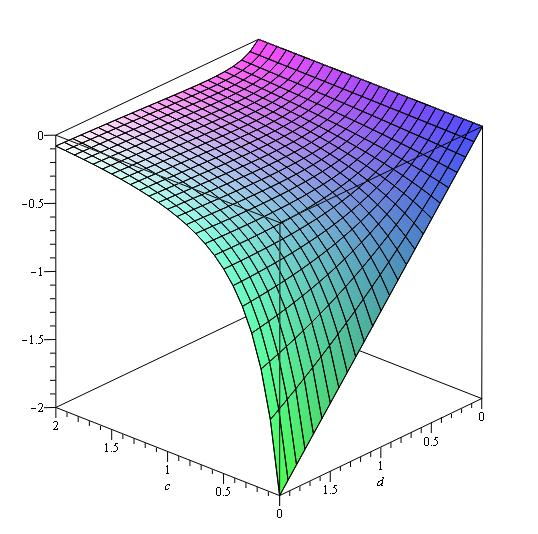
\includegraphics[width=0.4\textwidth]{ChapterFramework/figures/delCostPartial_C}}
 \hspace{0.1}
 \subfloat[$\frac{\delta Y}{\delta d} = - \frac{w\cdot c}{(1+c\cdot d)^2}$]
{\label{fig:partialdel2}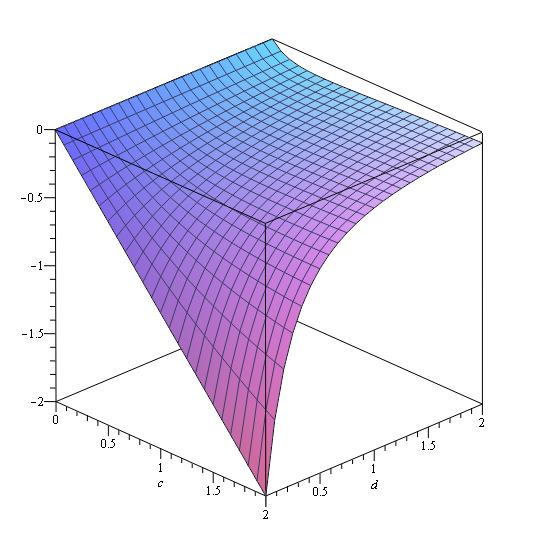
\includegraphics[width=0.4\textwidth]{ChapterFramework/figures/delCostPartial_D}}
\caption{Graphs of partial derivatives for $c$ and $d$ from $Y = w / 1 + c \cdot d$. Graphs assume $w=1$. \label{fig:delcostpartials}}%
\end{figure}

Allowing $w$ to be one, these are graphed in figure \ref{fig:delcostpartials}. Consider $\delta Y/\delta d$ (figure \ref{fig:partialdel2}) first: how distance $d$ changes `what I can buy with my wage', holding distance cost $c$ constant. Take $c = 0$: with no delivery cost, distance itself does not change what I can buy: space has no impact. As $c$ increases, however, $d$ has a larger impact earlier on, and the dropoff is steeper as the delivery cost goes up. So, where $c = 2$ and $d = 2$, there's much less of a drop in what I can buy with my wage if I change either of them.
 	 	 
$\delta Y\delta d$ (figure \ref{fig:partialdel1}) is structurally exactly the same, but highlights a slightly different point. 

What it's saying: look at where d is 2. What's happening with c? Well, "the amount I can buy with my wage" decreases much more rapidly for changes in smaller quantities of delivery cost than larger. 
OK: so that should all explain why we get this:
That's with density costs set to zero. Interestingly the shape wasn't so different with density costs present - oh, that would be because people can't move and their location is evenly spread: the cost will be the same for all of them, pretty much.
OK, just spent some time wiggling the delivery cost in the vis and I think I get it now - particularly for dy/dc. The changes are much more rapid for the those further away as dc increase. The change - proportional to what is much smaller utility - as they become high is much, much smaller.
So if we're imagining a Glaeser-like situation where transport costs are very low, that's interesting: it's possibly saying, changes in transport costs when they're low will have a larger impact than shifting between already-high transport cost-areas. 
I think partial diff might be magic. 
Except that doesn't account for transport costs as a \% of base price. I think (though am checking below) it's going to mean: changes in transport costs in low-transport cost situations will affect low value density cost goods more than high value. Which is intuitive enough, if you've managed to hold onto all the bits of that to the end of this sentence.



Within the limitations of partial analyses, agent-based actors do still find optimal spatial outcomes of interest. This section outlines the most interesting from within the model framework. 

%What's good about density cost is it allows me to concentrate on thinking about this spatial equilibrium problem without worrying too much about, say, rent structure or where that money goes. It's a bit like iceberg transport costs in that respect.

\section{`Backyard' models \label{sec:backyard}}

%To recap, the space cost variables to be examined are: distance, time, factors and utility. The first model iteration -  the 'backyard' models - looks at the first three of these. In this model, time is the only factor, and each actor must decide how best to spend their time, splitting it between movement and production. 

\input{ChapterModels/Tables/modelatom_backyard_table}

The `backyard' model is the counterpart to the single-actor love-of-variety trade model outlined in section \ref{sec:modelatom_increts}. That model found that a single actor type, with linear production, could trade over space purely through love of variety. The backyard model is the counterpoint: in a single-actor world, with \gls{increts} in \emph{production}, what are the minimum conditions that will get them out of their backyard?

The basic choice facing actors is the same: are there more productive options than producing in my own backyard, where output is linear with time input? Every actor is set up such that, if more time is input into their production, \gls{increts} can be gained. Thus there is an incentive - for example - for two actors to collaborate at one site and split the productive proceeds. 

An immediately obvious difference to the love-of-variety trade model is the nature of the indivisibilities. Whereas trade does not have to happen where goods are produced,actors combining labour must do so at a particular site of production. The barrier in the way of collaboration, then, is the cost for actors to get to the site of production.

There are two elements to the model it is worth discussing in more detail before getting on to the results. Firstly, as mentioned in the table, time is the only factor.
\cmt{model component tables: don't currently list types of good or productive factor. They probably should.}
This is similar to the core model, where labour is the only input. The difference here is that time must be spent between production and space.

Secondly, the model begins with actors of uniform type: there is no initial distinction made between consumers and producers. This is a departure from the standard \gls{ge} assumption of a world where consumers and firms are defined separately. 



\section{Comparing constrained and greedy utility}

%%%%%%%%%%%
% Brute force vs analytic
%%%%%%%%%%%
%As discussed, the two-good models use an `Engel function' able to either act as a Cobb Douglas if $\gamma$ is set to zero, or to distinguish the two goods as necessity and luxury (see section \ref{sec:utilitynengelslaw}) . 
%In an analytic setting, using  constraints (equations \eqref{eq:engelsmurataFopt} and \eqref{eq:engelsmurataFopt}) would be normal. 
As discussed above, for a given budget and set of prices, equations can be deduced that say precisely what the optimal quantity of goods should be. In an agent setting, it is possible to find optima through brute computational force: simply search the entire parameter space and keep whichever produces the highest utility. This is, of course, more computationally expensive than using a simple constrained optimisation equation, so it is a natural step to wonder whether those equations can be used instead of a brute force approach. The answer, surprisingly, is no. 
%Section \ref{sec:blackbox_tel} picked up on some of Hayek and Jacobs' arguments that gave a background to why this might be so. Here, some modelling reasons that support their argument are discussed.

Consider three options for an actor finding its maximum utility - brute force, or one of two constrained optima, the first constrained by a given total quantity of the two goods, the second including the price of both goods. In the brute force approach, the actor searches a range of possible mixes of $F$ and $M$ in Cobb Douglas utility function \eqref{eq:-3} to find the optimal mix:

\begin{equation}
max\; U=F^{\delta}M{}^{1-\delta},\; (0<\delta<1),\; F+M=Y
%U=F^{\delta}(M+\gamma){}^{1-\delta},\; (0<\delta<1),\; \gamma\geq0,\; F+M=Y\label{eq:engelsmurata2}
\end{equation}

As discussed earlier, for a budget of $F+M=Y$, the non-price constrained optima for the two goods is:

\begin{equation}
F=\delta Y
%F=\delta(Y+\gamma)\label{eq:engelsmurataFopt2}
\end{equation}

\begin{equation}
M=(1-\delta) Y
%M=Y-\delta(Y+\gamma)\label{eq:engelsmurataMopt2}
\end{equation}

Including price, the optima are as follows ($p_F$ and $p_M$ are the price of $F$ and $M$ respectively).

\begin{equation}
F=\frac{\delta Y}{p_F}
%M=\frac{Y(1-\delta)}{p_{M}}-\delta\gamma\label{eq:engelpriceoptM}
\end{equation}
 
\begin{equation}
M=\frac{(1-\delta) Y}{p_M}
%F=\frac{\delta Y-Y+\delta\gamma p_{M}}{p_{F}}\label{eq:engelpriceoptF}
\end{equation}

So why can't either two of these constrained optimisations be used? It is impossible to assume that goods will be available to meet a set `objective' demand. Consider what people must do (outside of the choice of backyard, which avoids all co-ordination problems.) They need to find information. Either -

\begin{itemize}
	\item How much of F or M can I get for my time?
	\item How much money can I get for my time, and how much of F and M will that buy?
\end{itemize}

Even if time or money can be used to produce an `objective demand', the model probably cannot supply it. The only option for people is to check what bundles of goods are available and test which mix is best. Compare this to equations \ref{eq:engelsmurataFopt2} and \ref{eq:engelsmurataMopt2}: both require prior knowledge of the budget, $Y$ - that is, the total quantity of goods. That `budget level' is not given - there is a wage, but not an `amount of $F$ plus $M$'. 

Graphs for MNND distance. Currently using many-run averages...

\begin{figure}
  \centering
 %\subfloat[A gull]{\label{fig:gull}\includegraphics[width=0.3\textwidth]{gull}}                
  %\subfloat[A tiger]{\label{fig:tiger}\includegraphics[width=0.3\textwidth]{tiger}}
  \subfloat[All actors]
  {\label{fig:bhg1}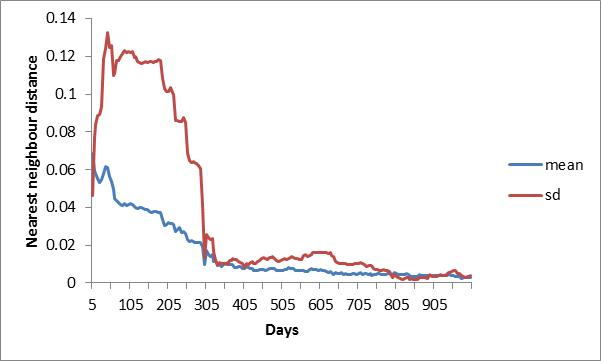
\includegraphics[width=0.4\textwidth]{ChapterFramework/figures/mnnd_blackholegraph1}}
  \hspace{0.2}     
  \subfloat[People]
  {\label{fig:bhg2}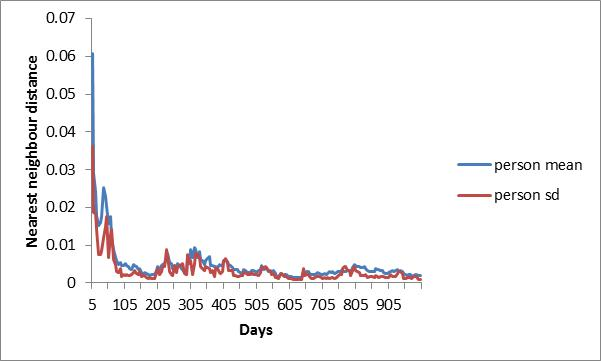
\includegraphics[width=0.4\textwidth]{ChapterFramework/figures/mnnd_blackholegraph2}}
  \hspace{0.2}  
  \subfloat[Firms]{\label{fig:bhg3}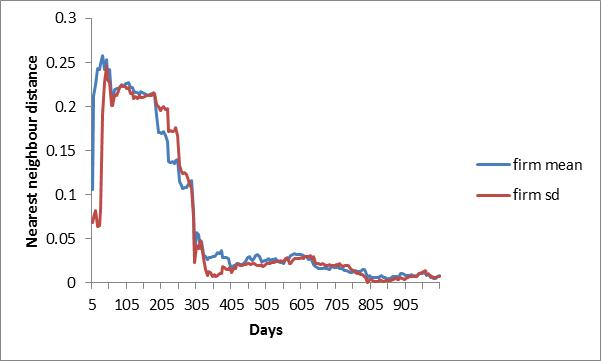
\includegraphics[width=0.4\textwidth]{ChapterFramework/figures/mnnd_blackholegraph3}}
  \caption{Mean and standard deviation of nearest neighbour distance, randomised starting locations}
  \label{fig:blackholegraphs}
\end{figure}

Bits from DMR
Five factors interact with Firms' ability to make a correct response in this situation. First, the decisions other Firms have taken will affect a Firm's revenue. Second, in this example People are using a CES utility: decreasing $\rho$ (thus increasing \gls{lov}) makes it less likely that other Firms' actions will impact on a Firm's revenue. There are then factors relating to how People's utility is structured. Where the constrained algorithm provides Firms with very precise price signal feedback, the greedy algorithm's relative lack of precision muddies the waters. As a result, the lower the number of iterations in the greedy algorithm, the harder Firms find it to improve their revenue. Lastly, Firms can use a method to deal with small-period turbulence in the revenue data: they simply take an average over a given period of days. 

Firstly:
Firms' ability to find their way to better revenue is dependent on a combination of: the actions of other Firms, and their own ability to interpret the data they get from the world correctly.Other Firm's actions can cause them to misinterpret their own action, and so make bad decisions. In this example, this slows down, but does not stop, their ability to improve their income. \gls{eosub} between goods (which is, from the point of view of People, \gls{lov}) affects the extent of this mismatch between data and interpreted meaning: one Firm can take a larger chunk of the other's potential revenue when \gls{eosub} is lower. 

Second, Firms can find a dynamic stability. (I think I've already written about this below somewhere.)
.. %\hspace{0.2}  
%\subfloat[]{\label{fig:dc_densitydist}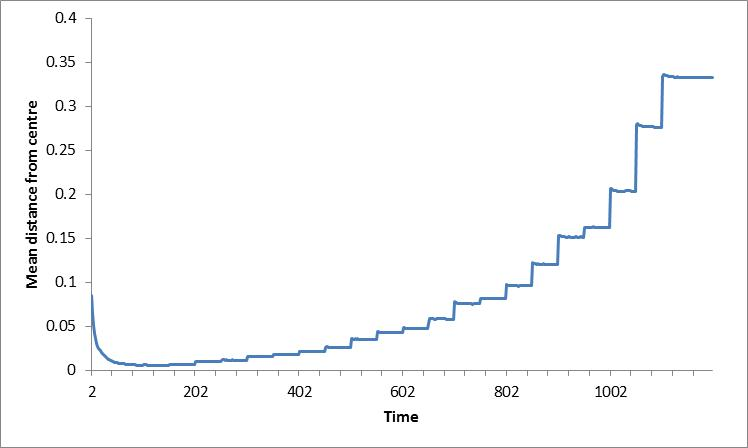
\includegraphics[width=0.4\textwidth]{ChapterFramework/figures/densitycost1/densityseq_meandistfromcentre}}

Spatial eq bits
"	Wage
"	Distance to Firm in time
o	Wage is proportional to time put in
"	Base good cost
o	Delivery cost per unit (dcost * distance), gets added to base cost
o	Note what happens with this delivery cost setup: as it approaches zero, goods become the same price everywhere. Space no longer matters for good cost.
"	Density cost
o	If we're using just two actors, defined for when they share a square.
"	Utility
o	Each person gets utility from good. Err� I presume that I can manage with linear utility, but I don't know if that's true. I should just check that� Yup, fine. Phew.
Greedy al bits. Same as framework. Keeping just in case


\begin{figure}%
\centering
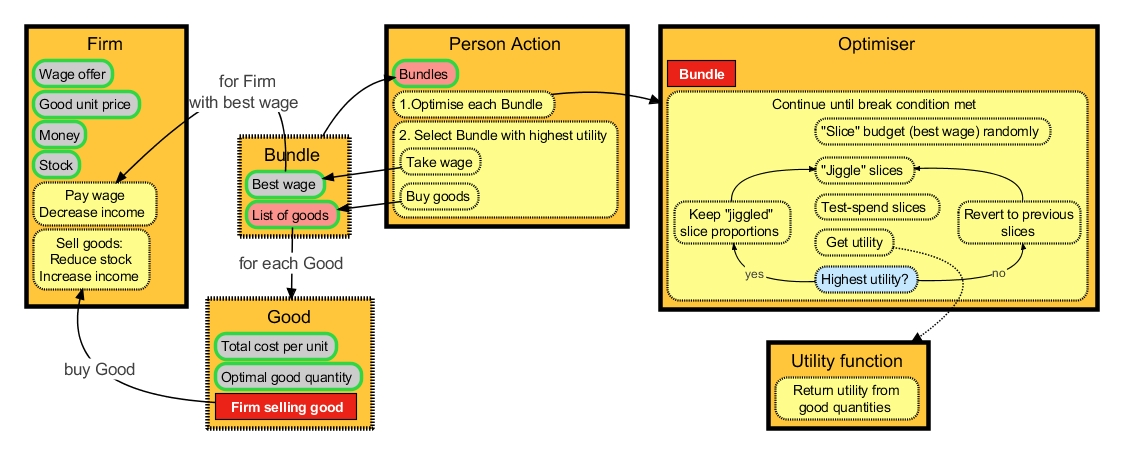
\includegraphics[width=1\columnwidth]{ChapterFramework/figures/PersonOpt}%
%\includegraphics[width=0.85\columnwidth]{ChapterModels/Figures/hillclimbExcel}%
\caption{Optimisation of Bundles in a Person's action}%
\label{fig:personopt1}%
\end{figure}

\begin{itemize}
	\item Optimise each Bundle. This happens in an Optimiser:
	\begin{itemize}
	\item The Optimiser iterates, either for a set number or until some condition is met (such as no marginal utility gain for a certain number of steps: see below.) 
	\item The iteration is initialised by randomly slicing the budget (the best wage), one slice for each Good in the bundle, before beginning the iterations. The iterations are:
	\item `Jiggle' the slices, changing their proportionate size slightly.
	\item `Test-spend' those slices on each Good: find out how much could be bought with the current budget slices using the per-unit price for the Good.
	\item Get a utility level for these quantities of goods. The Utility function is logically separate: the Optimiser deals only with this process of random slicing and adjusting.
	\item If the utility level found is the highest so far, keep the current proportion of slices and return to the 'jiggle' point. Else, revert to the previous slice proportions and try again. This has the effect of ratchetting the budget slices (and thus the spend per Good) towards an optimum.
	\end{itemize}
	\item Once each Bundle has an optimum utility, select the Bundle with the highest:
	\begin{itemize}
	\item Take the best wage: this instructs the Firm to pay the Person.
	\item Buy goods in the quantities found optimal by this Bundle.
	\end{itemize}
\end{itemize}

Figure \ref{fig:CESHillClimbIllustration} graphs data from this process in action. A bundle containing sixteen goods of equal cost is optimised for a CES function over a thousand iterations. (The optimum for a CES function with equal-value goods is  already known from section \ref{sec:CESbasics}: an even mix.) In this example, the optimum is found quite slowly: this helps to illustrate the process. The first graph shows initially random budget split guesses converging on the optimum mix of $0.06$ for each good. The second shows the marginal utility gain from each iteration; most of the gains happen very quickly, after which almost no extra benefit accrues (though there is a very small amount of further convergence.)

The important difference to analytic constrained optimisation is that people can work with any number and type of good and can deal with limited stock levels.
\cmt{Need to illustrate what happens in limited stock situations, what happens to money if it can't all be spent.}
If People find an optimal amount simply isn't available to them, they must spend their wage accordingly. 

\cmt{somewhere: need to compare this limited notion of rationality with the critiqued `superhuman' rationality that conflates the ability to tell better from worse with perfect knowledge of the whole market. Also, the `realism' of 1000 iterations for finding utility. Here probably isn't the place. Also x-ref to Fowler's agent model, which uses objective optima, and Firms can use that signal.}

\begin{figure}%
\centering
\includegraphics[width=0.85\columnwidth]{ChapterModels/Figures/hillclimbExcel}%
\caption{Utility-maximising stochastic search algorithm, optimising a CES function with 16 goods over a thousand iterations (x axis)}%
\label{fig:CESHillClimbIllustration}%
\end{figure}
...
Cut comments
\cmt{Should also write up: `lock-in' effect when many actors are on same spot; each reinforces the location of the other. Once formed, the exact location of a black hole point will not change/drift unless perturbed.}
\cmt{MNND: meaning of SD is different in spatial context. These are perhaps placeholders, while we get text done, then work out what needs more detail and of what sort.}
...
DMR
But are these appropriate responses? This depends on whether the Firm is correctly interpreting their data - and in a competitive situation, they may not be. Given that all parameters are fixed, there are only two ways a Firm can increase revenue: reducing delivery costs by being closer to their market, or taking trade away from another Firm. It is this last point that presents problems for the Firm's understanding of the data: revenue may have dropped, but it may not be because of the action the Firm has taken. If they then reverse that action, this is an \emph{in}appropriate response, based on misunderstanding of the data.
Kind of true, but if space is involved, problematic. Though also if they were changing price, it would be too: 
When actors have love of variety controlled through $\rho$, this also dictates how directly Firms will be competing. When $\rho=1$, goods are perfect substitutes, and Firms can only compete on cost (which in this scenario, they can only reduce by getting closer to their market.) As $\rho\to0$, people increasingly prefer a mix of goods - but it also has a surprising effect on Firms: they find it easier to discover the optimal location. Where they are competing more directly, however, the problem of faulty data is strongest. A Firm will more often find their revenue has decreased.
This is intuitive enough: as goods become more complementary, and people want a mix of the two, a Firm's actions are likely to be correct, and the other Firms' actions won't be so prone to giving false negatives because they won't impact on the others' revenue so strongly.
The idea that the noisy demand of large numbers of People can average out, however, has to be based on an underlying similarity in tastes: the utility function is there, it is just more or less hard to uncover. But of course that is quite an assumption: people's tastes may change. 
...


In scenarios where People have a fixed wage \gls{lov} utility-maximisers' basic spatial outcome is intuitive: the location actors find is central to a given cluster. However, an interesting discrete outcome arises as a result of the rapid drop-off of demand for any one good as costs increase.

..

Like the Cobb Douglas, the Constant Elasticity of Substitution function sets up a situation where all goods of equal price enter into utility equally, regardless of the level of income. Spatially, one of the consequences of this is that the choices facing actors actually do not change as costs increase. Utility may drop, but discrete decisions about which firm to work for will remain the same, since the reasons behind those choices cannot change. 


\begin{figure}%
\centering
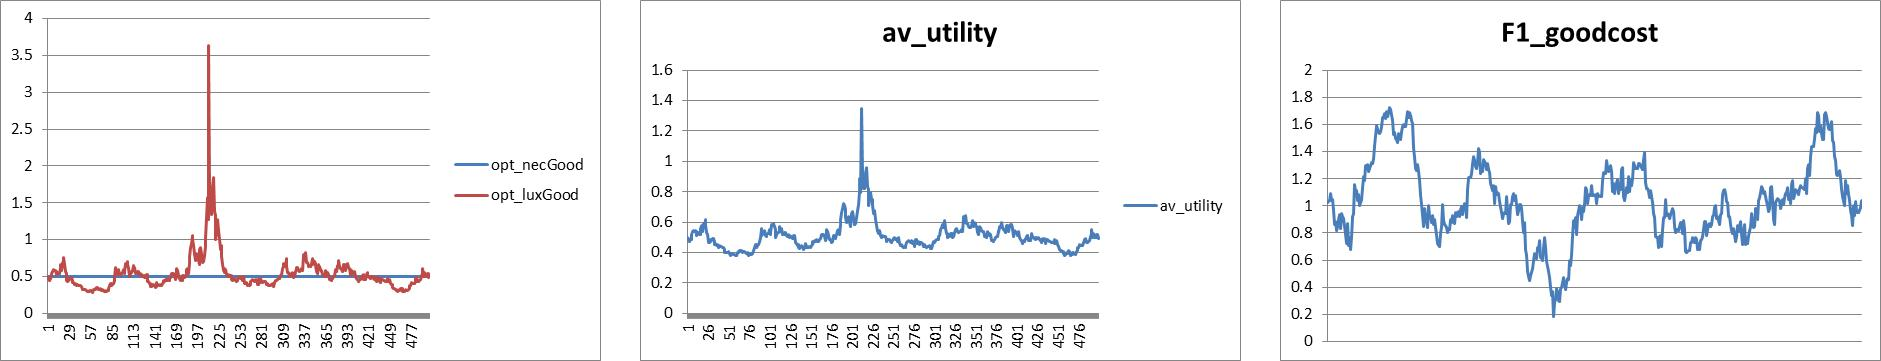
\includegraphics[width=0.85\columnwidth]{ChapterFramework/figures/CD_1fixed}%
\caption{Two firms, Actors with Cobb Douglas utility, one firm's price fixed.}%
\label{fig:CD_1fixed}%
\end{figure}
Any change in the cost of one good, therefore, does not affect demand for the other; this can be seen from the optimised demand equations \eqref{eq:engelpriceoptM} and \eqref{eq:engelpriceoptF}, which each contain only the price of their own good type. 
%The flipside of this is that, because demand for the two goods is completely independent, the total revenue flowing from demand for each cannot change. 


this robs Firms of any way to take action to change their revenue levels. 
In an agent context, however, this means that Firms collectively receive all the income from People (i.e. none leaks away through space costs), this removes the ability of Firms to make optimising decisions. This happens because, if all demand in the economy goes to Firms (so none `melts away' on delivery costs), revenue for each `sector' defined by the share parameter will not change. 
Figure \ref{fig:engelCorrection} illustrates this point: the uncorrected optima can lead to negative demand for the luxury good. Considering the equation for that good, this is unsurprising: $M = (Y(1-\delta)/P_m) - \delta \gamma$. Note that only the price for the luxury good enters into that equation, not the necessity good price. 
Figure \ref{fig:engeltest_income1to2} shows actors using the greedy algorithm to optimise the Engel function, reproducing the dynamic discussed in section \ref{sec:utilityengelslaw}.
...

Figure \ref{fig:transpace1} illustrates a simple spatial outcome from this approach, with Actors fixed to locations on a line. All trade with each other, producing a curve of utility with those near the centre better off. 

\begin{figure}[h!]
\centering
\includegraphics[width=0.7\textwidth]{ChapterModels/Figures/TransmissionSpace1cropped}}
\caption{Fixed Actors, delivery costs, finding efficient production levels. Red / high squares indicate higher utility. \label{fig:transpace1}}%
\end{figure}


%No circulation of money: the total flow of input is set and so can be considered the numeraire
%a way to make 'buying wage with time' work. 
%Some questions arise from that. Firstly, what counts as `too low or high' stock levels? The value is, in a sense, arbitrary. Zero is chosen as the target, but as x shows, if one is concerned to avoid economically unfeasible negative stock levels, a higher target value can be set. This can then be reached through price adjustments, leaving a `buffer' between the target value and zero.
%The value $P_1$ in this model is the `cost' in Actor 2's input $i_1$ for a unit of Actor 1's output. Actor 1, however, only has control over the base price $p_1$. 
%\begin{figure}[h!]
%\centering
%\subfloat[]
%{\label{fig:dc_util1}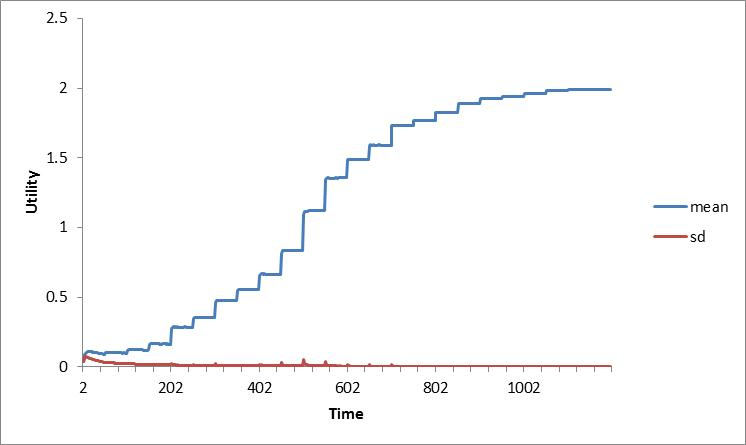
\includegraphics[width=0.4\columnwidth]{ChapterFramework/figures/densitycost1/densityseq_utiilty}}%
%\hspace{0.2}  
%\subfloat[]{\label{fig:dc_util2}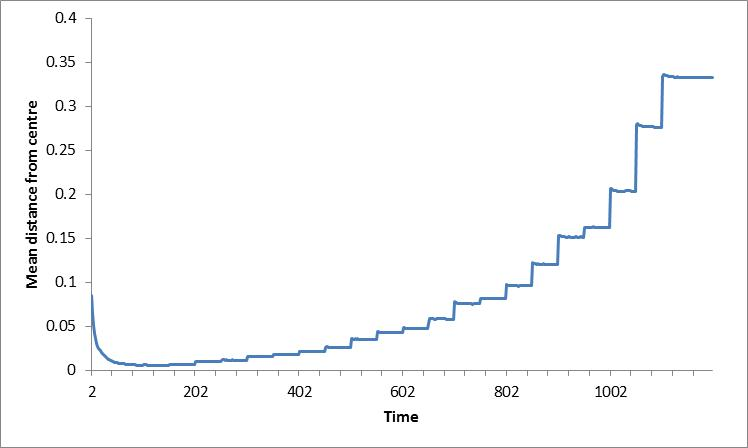
\includegraphics[width=0.4\textwidth]{ChapterFramework/figures/densitycost1/densityseq_meandistfromcentre}}
%\caption{Spatial equilibrium test. Utility and mean distance from centre as good space-cost is decreased. Utility standard deviation shows equilibrium. \label{fig:spatialeq2}}%
%\end{figure}
..
Each increase in mean utility is triggered by a decrease in good space-cost, and \ref{fig:dc_util2} illustrates that each of these leads to a larger spatial reach for all People. 
The important part of \ref{fig:dc_util1} is the standard deviation: it remains close to zero regardless of the space cost. Utility levels for all People quickly equalise. This is a spatial equilibrium outcome - all People are ending up with the same utility levels by self-organising in space. 
%Again, rubbish last sentence!
%This agent-based spatial equilibrium result is in some senses simpler than the kind of equilibrium found in urban economic models, and in other senses more complex. Taking each of these in turn: it requires only minimal rules and few things need be imposed exogenously. The result that utility ends up the same emerges from those rules. In comparison, a classic urban monocentric model is built on assumptions about bid-rent curves...
...
%There are situations where, while a spatial equilibrium is reached in the sense that no Person is able to move, it is not always a \emph{utility} equilibrium. Those with lower utiltiy would like to improve it, but path dependence in the model means some have superior positions, and it is not in their interests to change them. Such a situation is shown in figure \ref{fig:DC_vs_utilSD}.
..
A more mathematical analysis is used in two types of situation. Firstly, many of the basic dynamics of the model are best communicated using an analytic approach. Secondly, when the model framework produced results that required further explanation. When the agent model outputted a particular outcome, was it due to Actors acting rationally? If so, what factors were at work? The framework proposed these questions, but a full answer took a more analytic approach. Where those results have been informative, they have been included in this chapter. As discussed in the conclusion, this is a happy synergy: the agent model helping to highlight possible lines of inquiry, and an analytic approach shedding further light on the issues. 
Perhaps an agent critique would start by pointing out the following: the greedy algorithm is still built on a neoclassical foundation, with the same underlying utility function. But this returns to arguments about utility: as section \ref{sec:rationality} discussed, if one accepts that treating actors as simply reacting to costs in defined ways is useful, then this is no argument against using utility-like ideas in building actor optimisation methods.
additional modelling efforts of greater sophistication, including a more balanced approach to negative  demand, increased options for building in stock-level interactions that don't  rely on demand signalling, and, as the greedy algorithm doesn't demand any  particular utility function, the option to replace the utility function with  others of a broader scope, for example based on taste.
Conversely, the `greedy' approach may be useful in circumstances beyond constrained utility functions, each of which needs to be put through the Lagrange method and then hard-coded. In contrast,
Reasons for failure tended to revolve around trying to treat physical quantities of goods or money as exclusive, rivalrous goods. This often, for example, would simply lead to all currency funnelling to one Firm. Assuming unlimited stock also does not work: if Firms are price-setters, they are able simply to price right at the zero-limit, producing brief moments of infinite demand.
Rather than discuss those models in any depth, section \ref{sec:prodtowelfare} presents a model that does allow Actors to successfully connect production to welfare. However, one particularly interesting attempt at coordination is discussed next, as it reveals something about the informational challenges facing the model's economic actors. 
...
\subsection{Is density cost realistic? \label{sec:densitycostrealism}}
%Mention the difference of these two also:
%weight /= dlm.actors.size();
%weight /= gl.numTotalActors;
%Critics of location theory attacked... Massey 74. Should that go here? Point also: Christaller ideas were in fact used for planning, so the critiques were actually partly justified: the modelers were making the virtual world mistake. Stuck this in conclusion. Or maybe it should go in virtual worlds? Yup, I stuck it there. Cross-ref here.

%Density cost is a `second nature' effect - it is entirely relative to the location of each Actor, not determined by absolute location. This might seem contrary to how actual land markets work: surely each parcel of land has a specific location? True, but the value of that land is not set, it is determined by demand. This helps explain how the density cost method manifests a spatial equilibrium outcome - but the model does this without having to assume exogenous rent levels that drop off from some central point.
%On ad valorem tax on wage: point being, if wage is higher, there would be more `demand for density' which would offset the ability to afford higher density. Again: a weak proxy, interesting for thinking through spatial issues. Maybe. It is all urban econs though, which is slightly terrifying.
%Ah OK: it does make a difference, but in an interesting way. If the density cost is imposed as an ad valorem tax on the wage, the spatial outcome doesn't alter if you change the wage - kind of obviously if you state it like that. So really that's probably a point for the section on the realism of the density cost: changing good cost does affect space in this situation, because the density cost effect is altered. 
%It's perhaps a little more fiddly than that. As the wage goes up, utility does rise: People can buy more than they could, as their post-density-cost wage is still higher. But the point is comparative choices: a Person is unable to improve their density cost situation, relative to other People, by moving. The spatial element of the wage, $tech$, still has the same effect however.
%Still curious: if you move, density cost will be higher, but your wage will be higher since you're closer. Oh - except no it won't, if wage distance is turned off. I should make clear that's what's happening. Your wage won't be higher: you'll just be incurring a higher density cost if you try to move there.
...

\end{comment}
